\documentclass[12pt,a4paper]{article}
\usepackage{amsmath, empheq, geometry, graphicx, hyperref, physics, rotating}
\usepackage[extrafootnotefeatures]{xepersian}
\settextfont{XB Zar}
\title{آونگ متصل به دیسک}
\author{صالح شاملو احمدی\\دانشگاه صنعتی شریف، دانشکده فیزیک}
\date{21 اسفند 1399}

\hypersetup{colorlinks=true, citecolor=cyan, urlcolor=blue}

\begin{document}
	\maketitle
	\begin{figure}
		\centering
		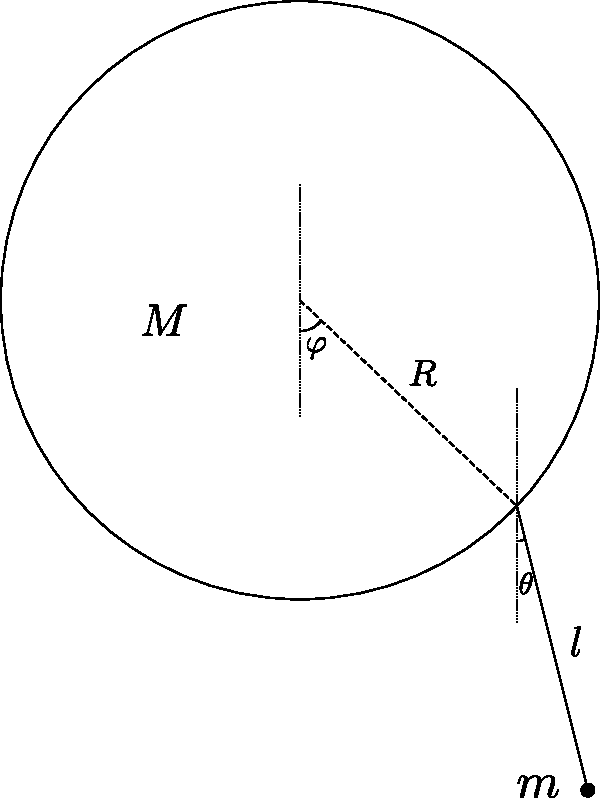
\includegraphics[width=\linewidth]{../figures/fig}
	\end{figure}
	\begin{abstract}
		در این نوشته حرکت یک آونگ متصل به یک دیسک به دیوار میخ شده را با استفاده از مکانیک لاگرانژی بررسی می‌کنیم.
		همچنین با حل عددی، مسیر حرکت آونگ را پیدا می‌کنیم و آشوبناک بودن یا نبودن سیستم را تعیین می‌کنیم.
		بررسی چنین مسئله‌هایی با مکانیک نیوتونی سخت‌تر است، چراکه باید نیرو‌های قیدی و شتاب دستگاه‌های نالخت خاص را حساب کنیم.
		با استفاده از مکانیک لاگرانژی کافیست انرژی جنبشی و پتانسیل را پیدا کنیم و ادامه حل فقط محاسبات ریاضیاتی است.
	\end{abstract}
	\section{معادلات حرکت}
	مختصات تعمیم‌یافته را زاویه ریسمان آونگ با محور عمودی و زاویه نقطه اتصال آونگ به چرخ با محور عمودی انتخاب می‌کنیم. داخل شکل این زاویه‌ها به ترتیب با $\theta$ و $\phi$ مشخص شده‌اند.
	
	برای بدست آوردن انرژی جنبشی، مختصات گلوله آونگ را در مختصات درکارتی پیدا می‌کنیم:
	\begin{empheq}[left=\empheqlbrace]{align}
		x(\theta, \phi) &= R\sin\varphi + l\sin\theta \\
		y(\theta, \phi) &= -(R\cos\varphi + l\cos\theta)
	\end{empheq}
	با مشتق‌گیری نسبت به زمان، سرعت را در دستگاه دکارتی پیدا می‌کنیم:
	\begin{empheq}[left=\empheqlbrace]{align}
		\dot{x}(\theta, \phi, \dot{\theta}, \dot{\varphi}) &= R\dot{\varphi}\cos\varphi + l\dot{\theta}\cos\theta \\
		\dot{y}(\theta, \phi, \dot{\theta}, \dot{\varphi}) &= R\dot{\varphi}\sin\varphi + l\dot{\theta}\sin\theta
	\end{empheq}
	حال انرژی جنبشی کل را پیدا می‌کنیم:
	\begin{align}
		T &= T_{\text{گلوله}} + T_{\text{دیسک}} = \frac{m}{2} \qty(\dot{x}^2 + \dot{y}^2) + \frac{I\dot{\varphi}^2}{2} \\
		&= \frac{m}{2}\qty[R^2\dot{\varphi}^2 + l^2\dot{\theta}^2 + 2Rl\dot{\varphi}\dot{\theta}(\cos\varphi\cos\theta+\sin\varphi\sin\theta)] + \frac{MR^2\dot{\varphi}^2}{4} \\
		&= \frac{m}{2}\qty[R^2\dot{\varphi}^2 + l^2\dot{\theta}^2 + 2Rl\dot{\varphi}\dot{\theta}\cos(\varphi-\theta)] + \frac{MR^2\dot{\varphi}^2}{4}
	\end{align}
	انرژی پتانسیل نیز فقط شامل انرژی گرانشی است:
	\begin{equation}
		U = mgy = -mg(R\cos\varphi + l\cos\theta)
	\end{equation}
	پس لاگرانژی برابر است با
	\begin{gather}
		\mathcal{L} = T - U \\ 
		\mathcal{L} = \frac{m}{2}\qty[R^2\dot{\varphi}^2 + l^2\dot{\theta}^2 + 2Rl\dot{\varphi}\dot{\theta}\cos(\varphi-\theta)] + \frac{MR^2\dot{\varphi}^2}{4}
		+ mg(R\cos\varphi + l\cos\theta).
	\end{gather}
	حال با استفاده از معادلات لاگرانژ، معادلات حرکت سیستم را پیدا می‌کنیم:
	\begin{empheq}[left=\empheqlbrace,right=\implies]{align}
		\frac{d}{dt}\pdv{\mathcal{L}}{\dot{\varphi}} - \pdv{\mathcal{L}}{\varphi} = 0 \\
		\frac{d}{dt}\pdv{\mathcal{L}}{\dot{\theta}} - \pdv{\mathcal{L}}{\theta} = 0
	\end{empheq}
	\begin{empheq}[left=\empheqlbrace]{align}
		\begin{split}
			&mR^2\ddot{\varphi} + mRl\qty[\ddot{\theta}\cos(\varphi-\theta) - \dot{\theta}(\dot{\varphi}-\dot{\theta})\sin(\varphi-\theta)] + \frac{MR^2\ddot{\varphi}}{2} \\
			&\hspace{12em} + mRl\dot{\varphi}\dot{\theta}\sin(\varphi - \theta) + mgR\sin\varphi = 0
		\end{split} \\
		\begin{split}
			&ml^2\ddot{\theta} + mRl\qty[\ddot{\varphi}\cos(\varphi-\theta) - \dot{\varphi}(\dot{\varphi}-\dot{\theta})\sin(\varphi-\theta)] \\
			&\hspace{12em} - mRl\dot{\varphi}\dot{\theta}\sin(\varphi - \theta) + mgl\sin\theta = 0
		\end{split}
	\end{empheq}
	\begin{empheq}[left=\empheqlbrace, box=\fbox]{align}
		& \qty(1+\frac{M}{2m})R\ddot{\varphi} + l\qty[\ddot{\theta}\cos(\varphi-\theta) + \dot{\theta}^2 \sin(\varphi-\theta)] + g\sin\varphi = 0 \\
		& l\ddot{\theta} + R\qty[\ddot{\varphi}\cos(\varphi-\theta) - \dot{\varphi}^2 \sin(\varphi-\theta)] + g\sin\theta = 0
	\end{empheq}
	\section{حل عددی}
	برای حل عددی، ابتدا معادلات دیفرانسیل را از هم جدا می‌کنیم:
	\begin{multline}
		\ddot{\varphi}(\varphi,\theta,\dot{\varphi},\dot{\theta}) =\qty[\sin^2(\varphi-\theta)+\frac{M}{2m}]^{-1} \bigg[\frac{g}{R}\qty(\sin\theta\cos(\varphi-\theta)-\sin\varphi) \\
		\left. - \sin(\varphi-\theta)\qty(\frac{l}{R}\dot{\theta}^2+\dot{\varphi}^2\cos(\varphi-\theta)) \right]
	\end{multline}
	\begin{multline}
		\ddot{\theta}(\varphi,\theta,\dot{\varphi},\dot{\theta}) = \qty[\sin^2(\varphi-\theta)+\frac{M}{2m}]^{-1}
		\bigg[\cos(\varphi-\theta)\qty(\dot{\theta}^2 \sin(\varphi-\theta) + \frac{g}{l}\sin\varphi) \\
		\left. + \qty(1+\frac{M}{2m})\qty(\frac{R}{l}\dot{\varphi}^2\sin(\varphi-\theta) - \frac{g}{l}\sin\theta) \right]
	\end{multline}
	
	دو معادله بالا بر حسب $\varphi$ و $\theta$ و مشتقات زمانی آنها، دو معادله دیفرانسیل مرتبه اول برای $\dot{\varphi}$ و $\dot{\theta}$ تشکیل می‌دهند.
	با ترکیب این دو معادله و معادلات ساده $d\varphi/dt = \dot{\varphi}$ و $d\theta/dt = \dot{\theta}$،
	یک سیستم معادله دیفرانسیل مرتبه اول برای $\varphi$ و $\theta$ و مشتقات آنها تشکیل می‌شود که می‌توان آن را به صورت عدد حل کرد.
	
	لازم به ذکر است که این دستگاه معادلات دیفرانسیل stiff\LTRfootnote{\url{https://en.wikipedia.org/wiki/Stiff\_equation}} هستند که باید در الگوریتم مورد استفاده برای حل، لحاظ شود.
	برای نمودارهای این نوشته، از روش BDF کتابخانه scipy زبان پایتون استفاده کرده‌ام.
	\section{نمودارها}
	نمودارهای مربوط به شرایط اولیه مختلف در صفحات بعدی هستند. با توجه به شکل نمودارها، واضح است که حرکت آشوبناک است.
	اما برای بعضی شرایط اولیه سیستم به یک حرکت نسبتاً پایدار و متناوب می‌رسد که اختلال کمی دارد.
	به طور خاص، برای حالتی که زاویه‌های اولیه کوچک باشند و نسبت جرم آونگ به جرم دیسک بسیار کوچک باشد، حرکت تناوبی ساده داریم.
	
	\newpage
	\pagenumbering{gobble}
	\newgeometry{left=0.125in, bottom=0.43in, right=0.125in, top=0.55in}
	\makebox[\textwidth][c]{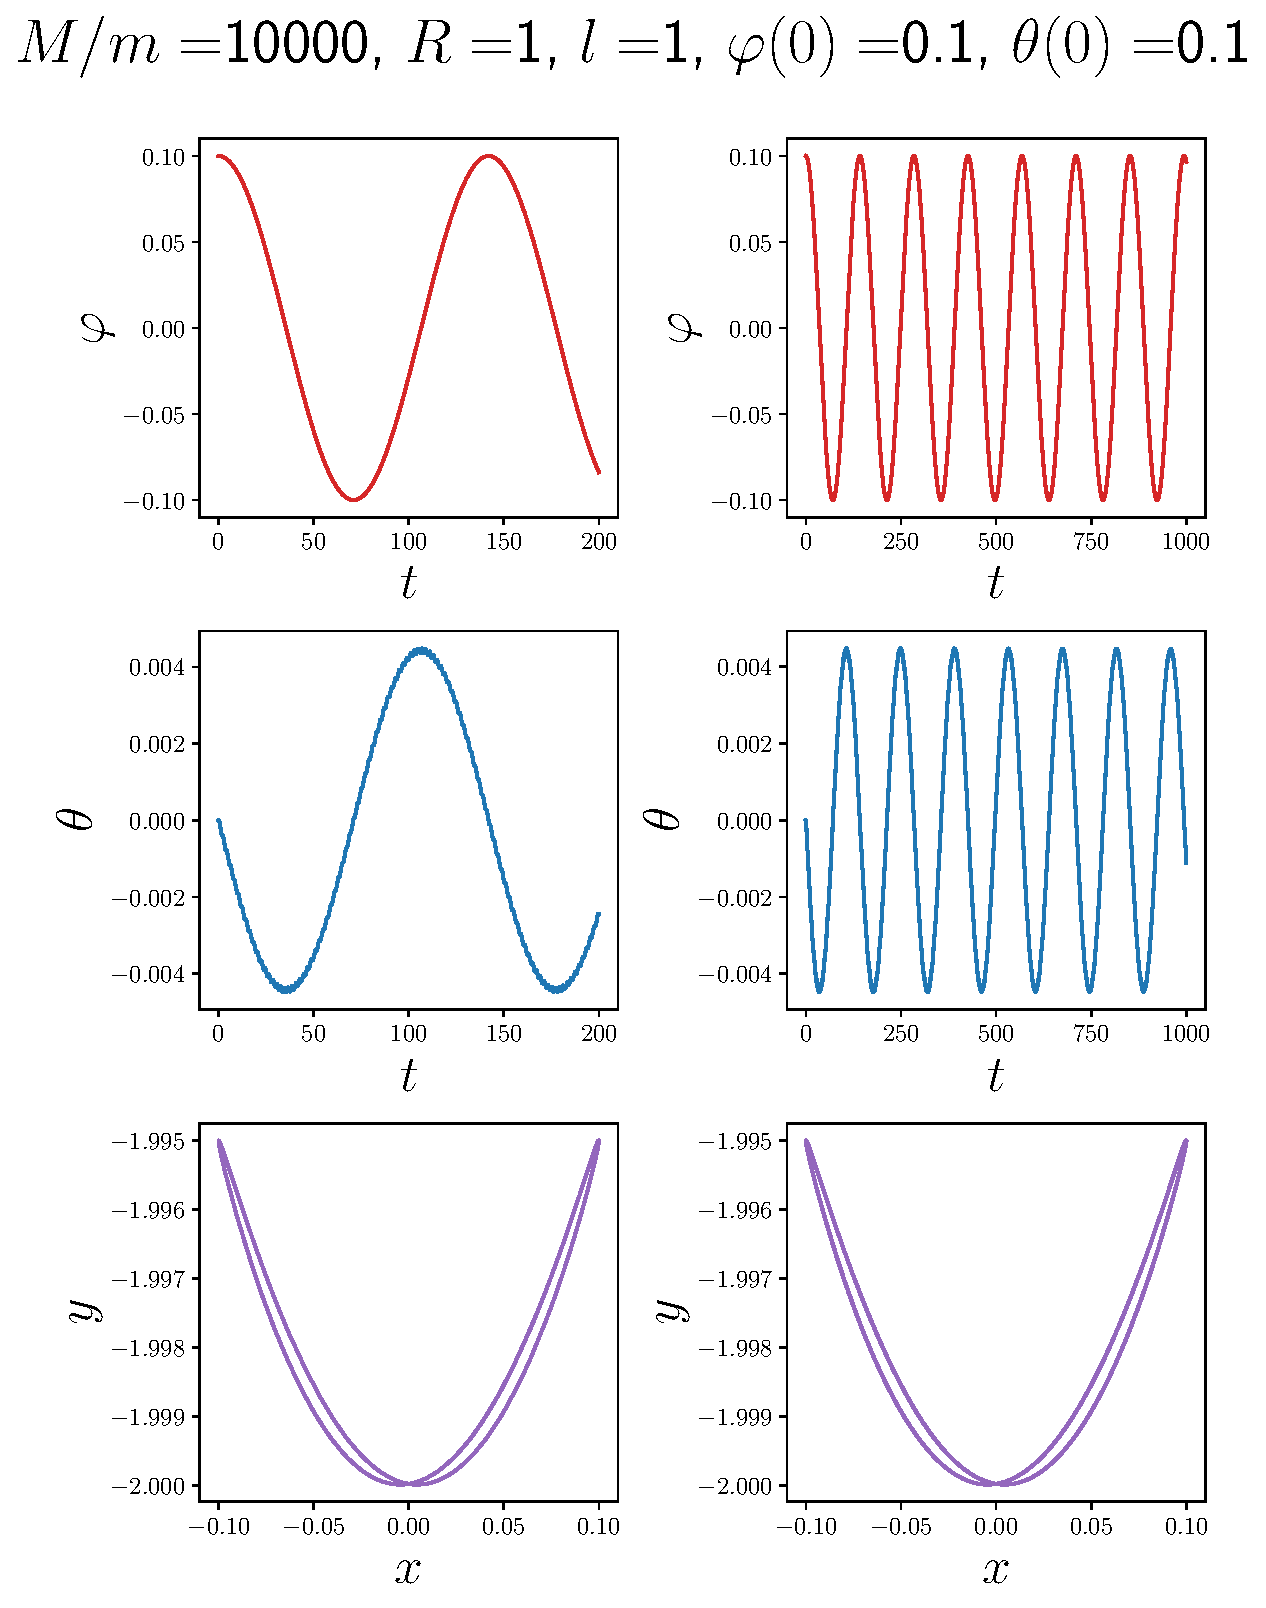
\includegraphics[scale=0.95]{../figures/0}}
	\makebox[\textwidth][c]{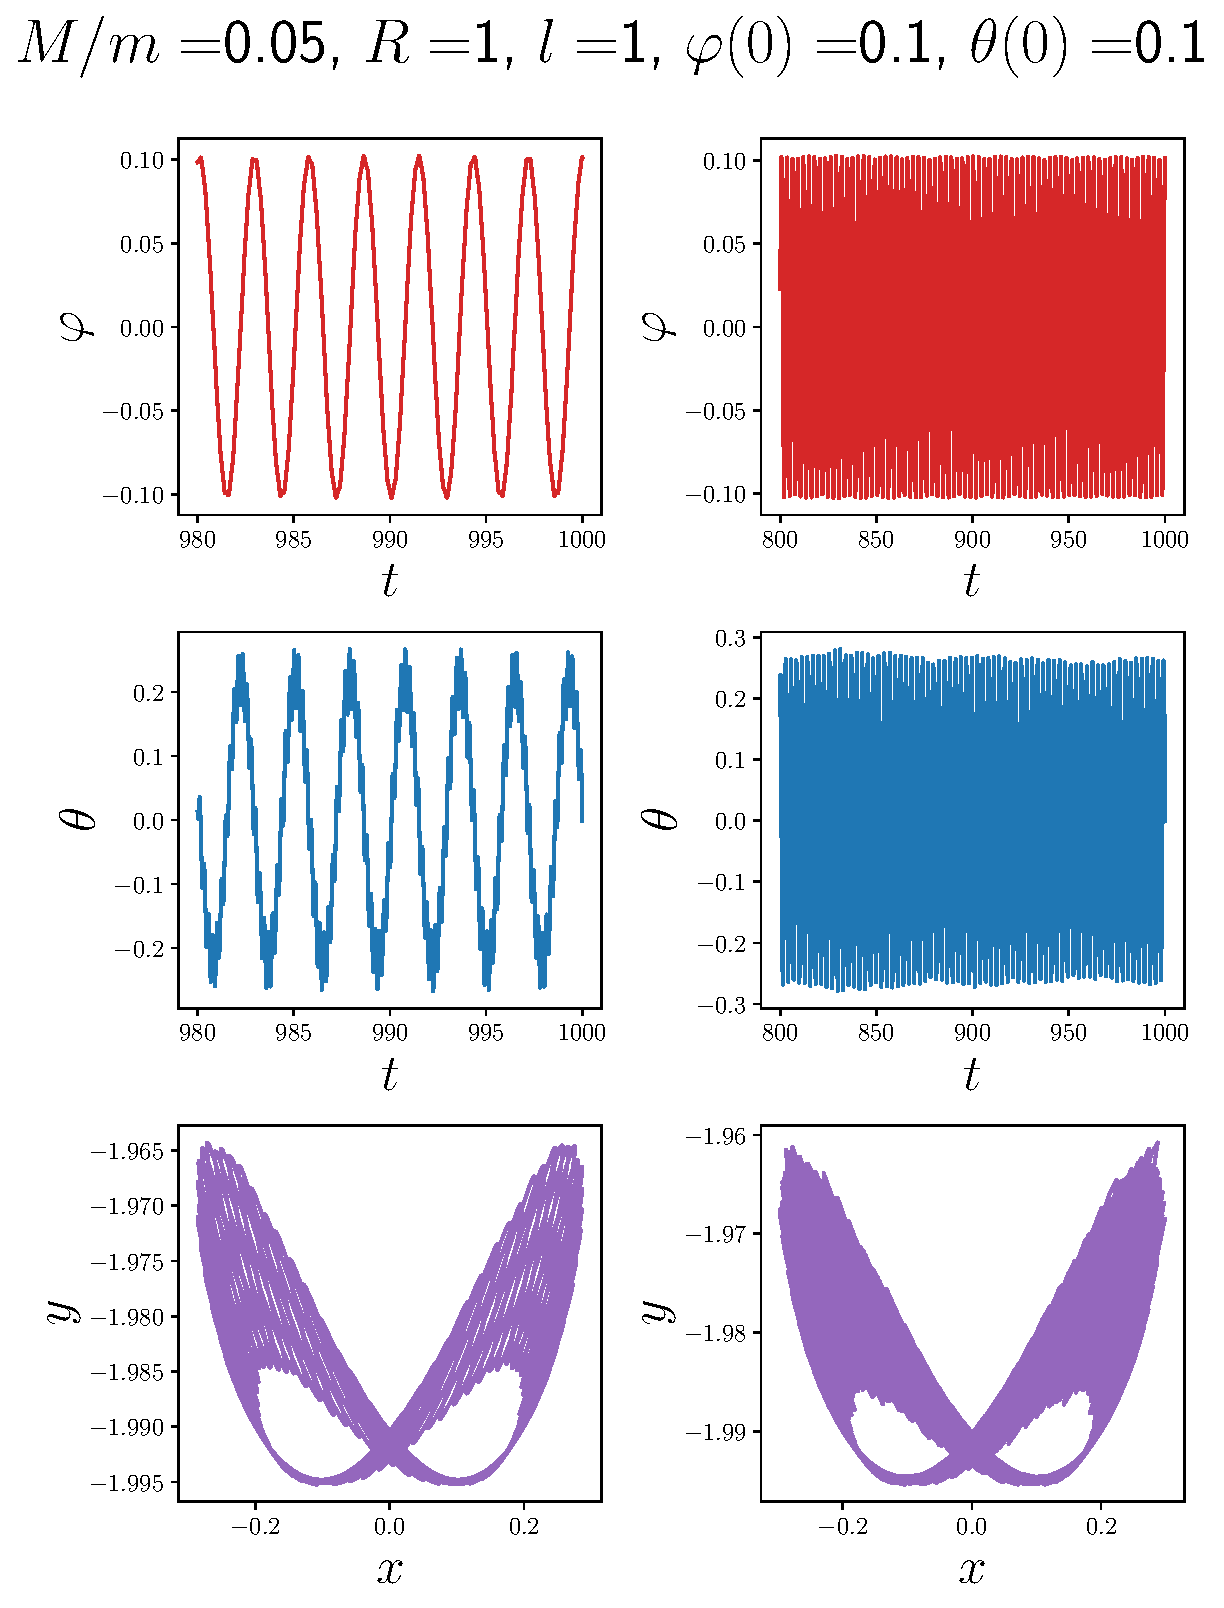
\includegraphics{../figures/17}}
	\makebox[\textwidth][c]{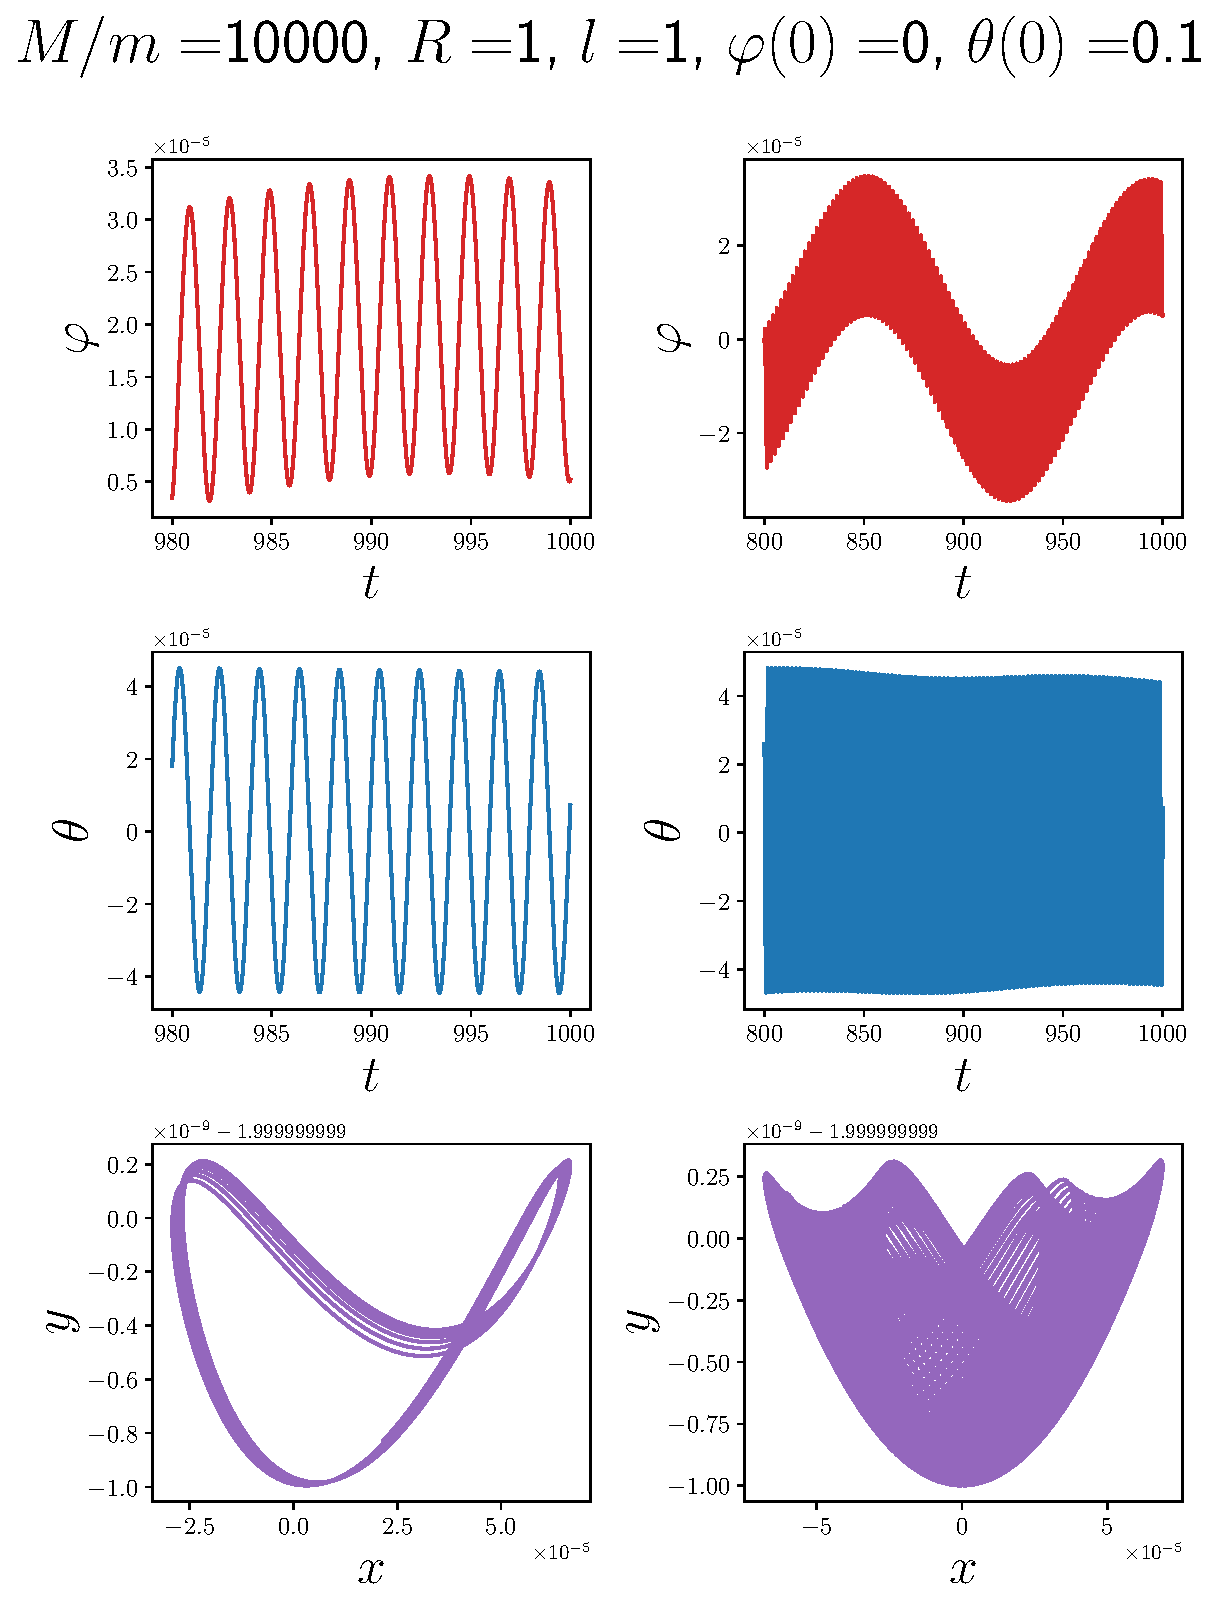
\includegraphics{../figures/s}}
	\makebox[\textwidth][c]{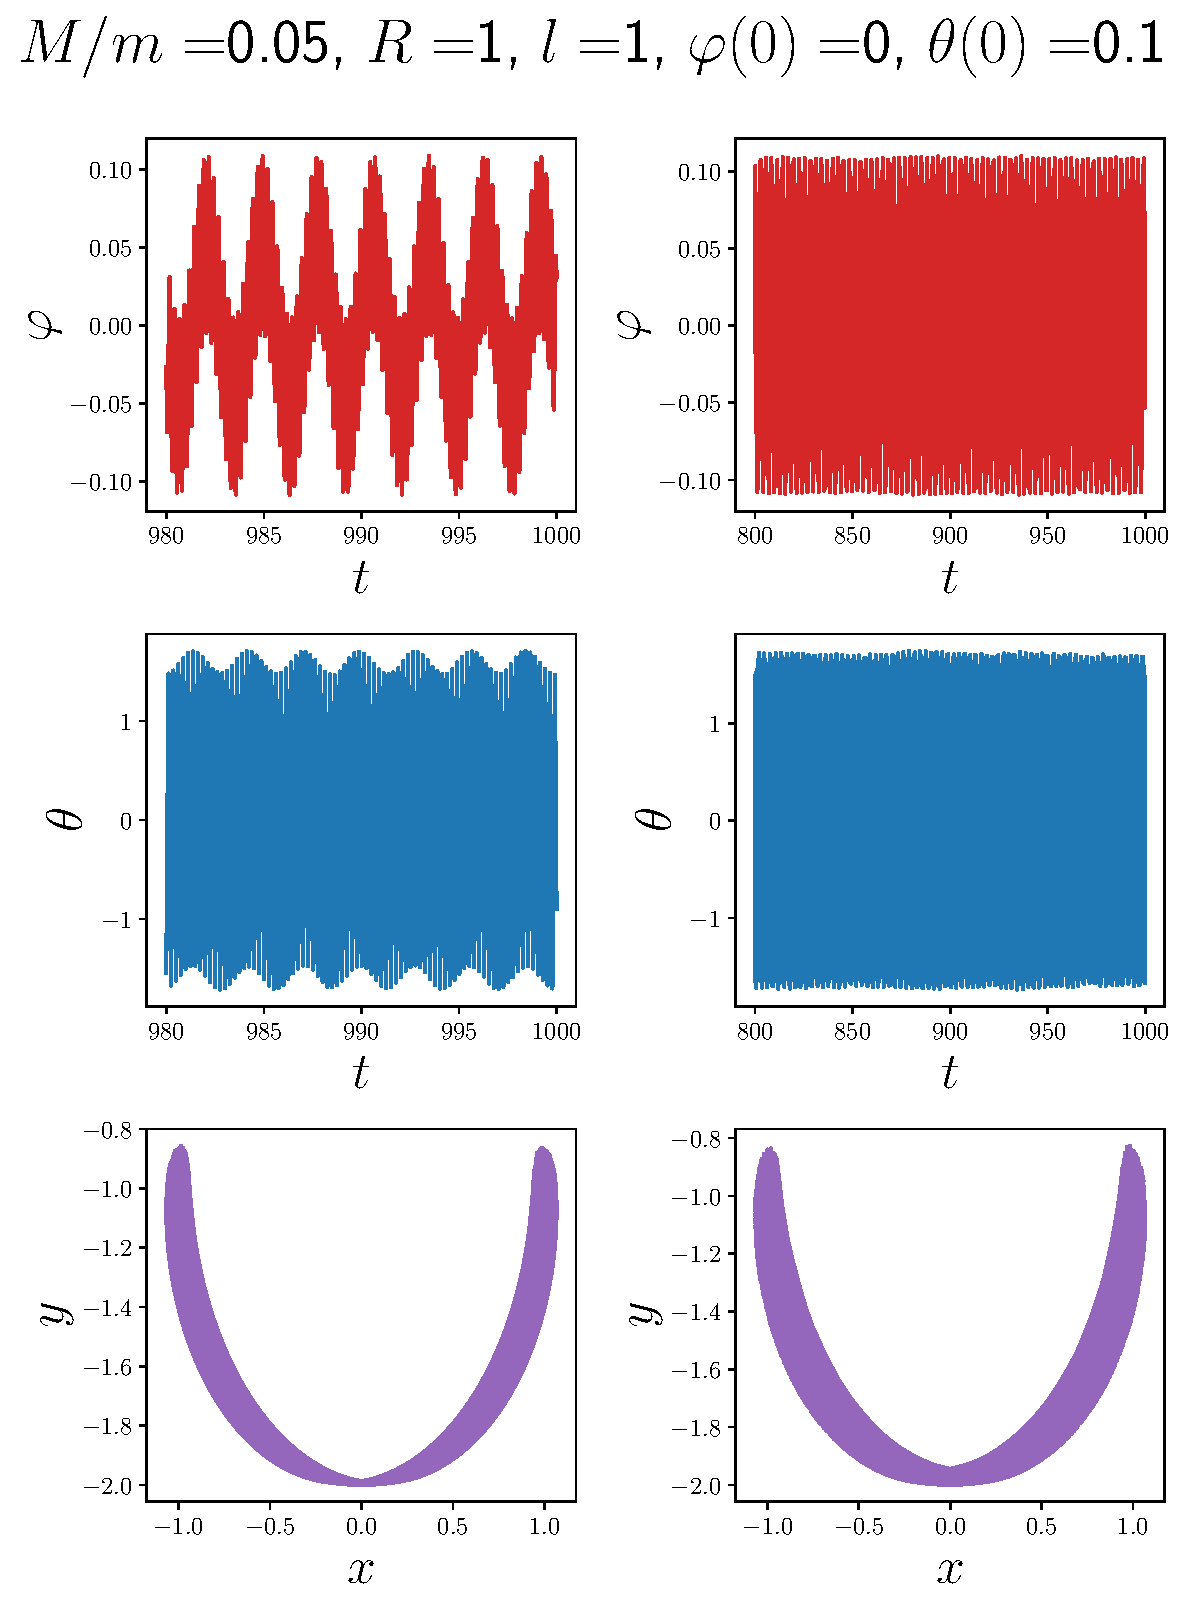
\includegraphics{../figures/b}}
	\makebox[\textwidth][c]{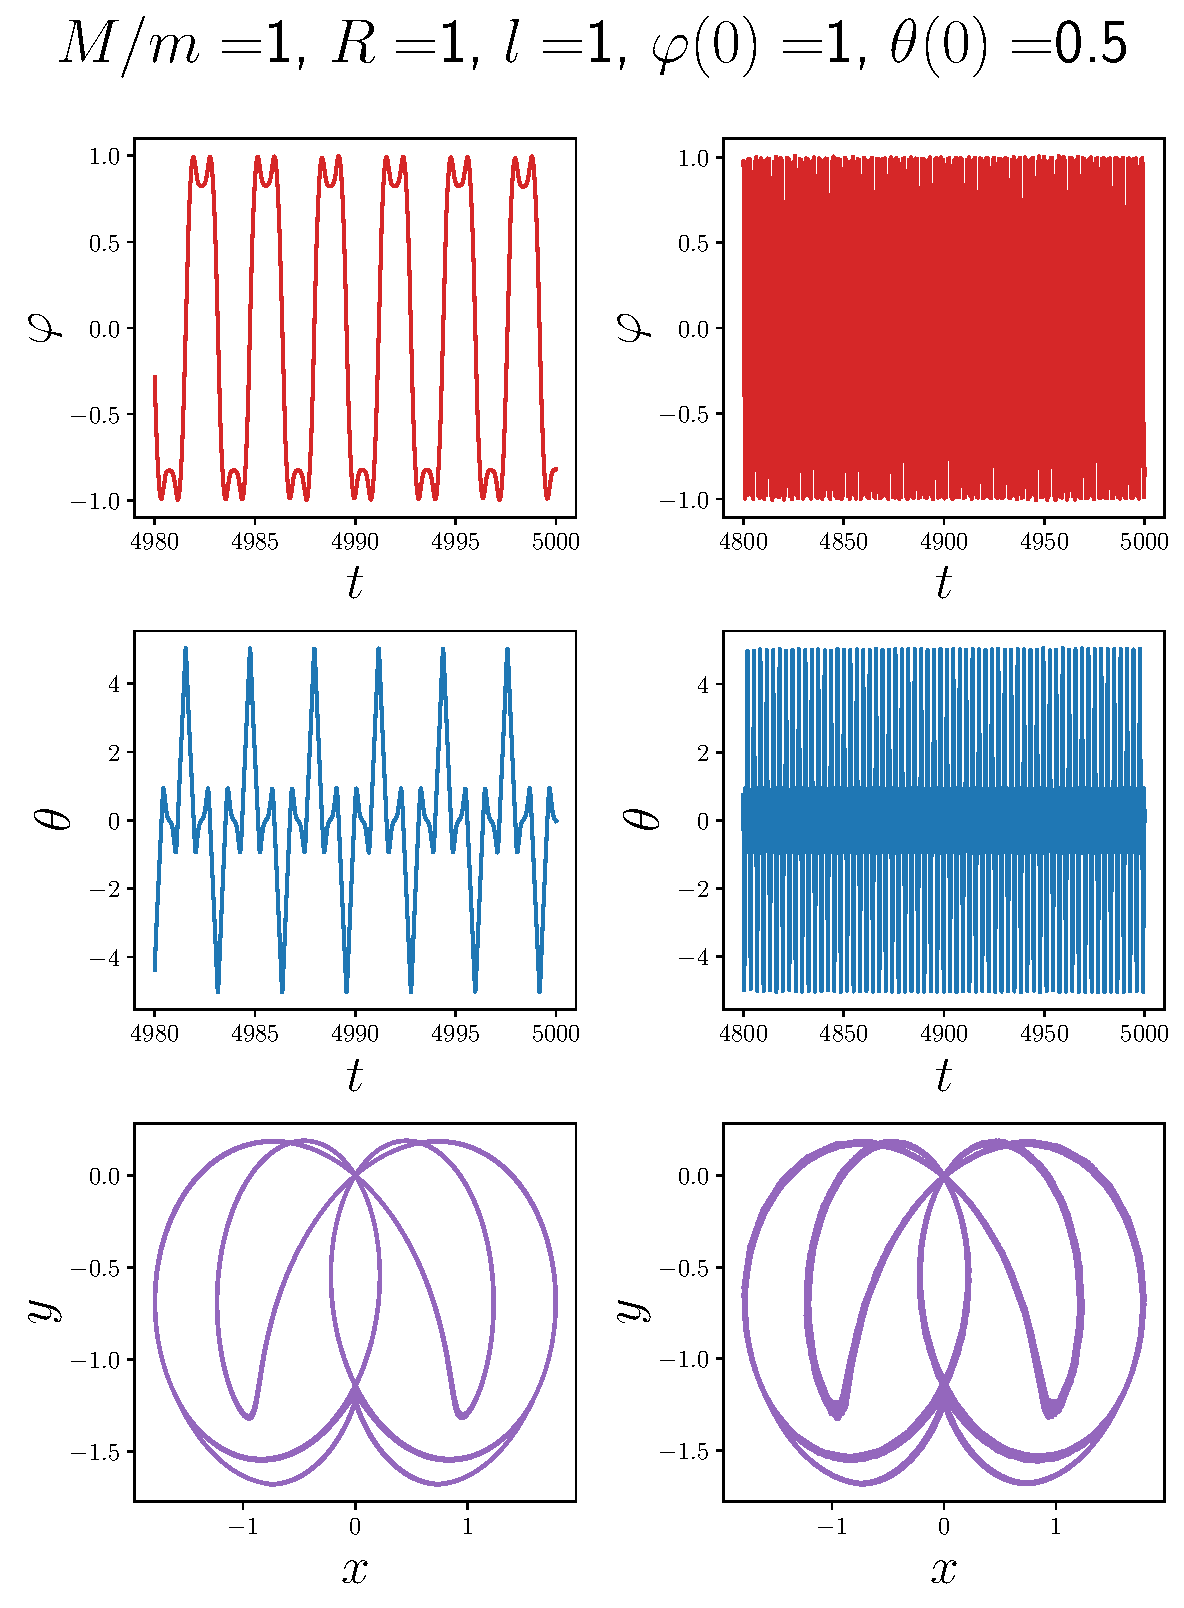
\includegraphics{../figures/1}}
	\makebox[\textwidth][c]{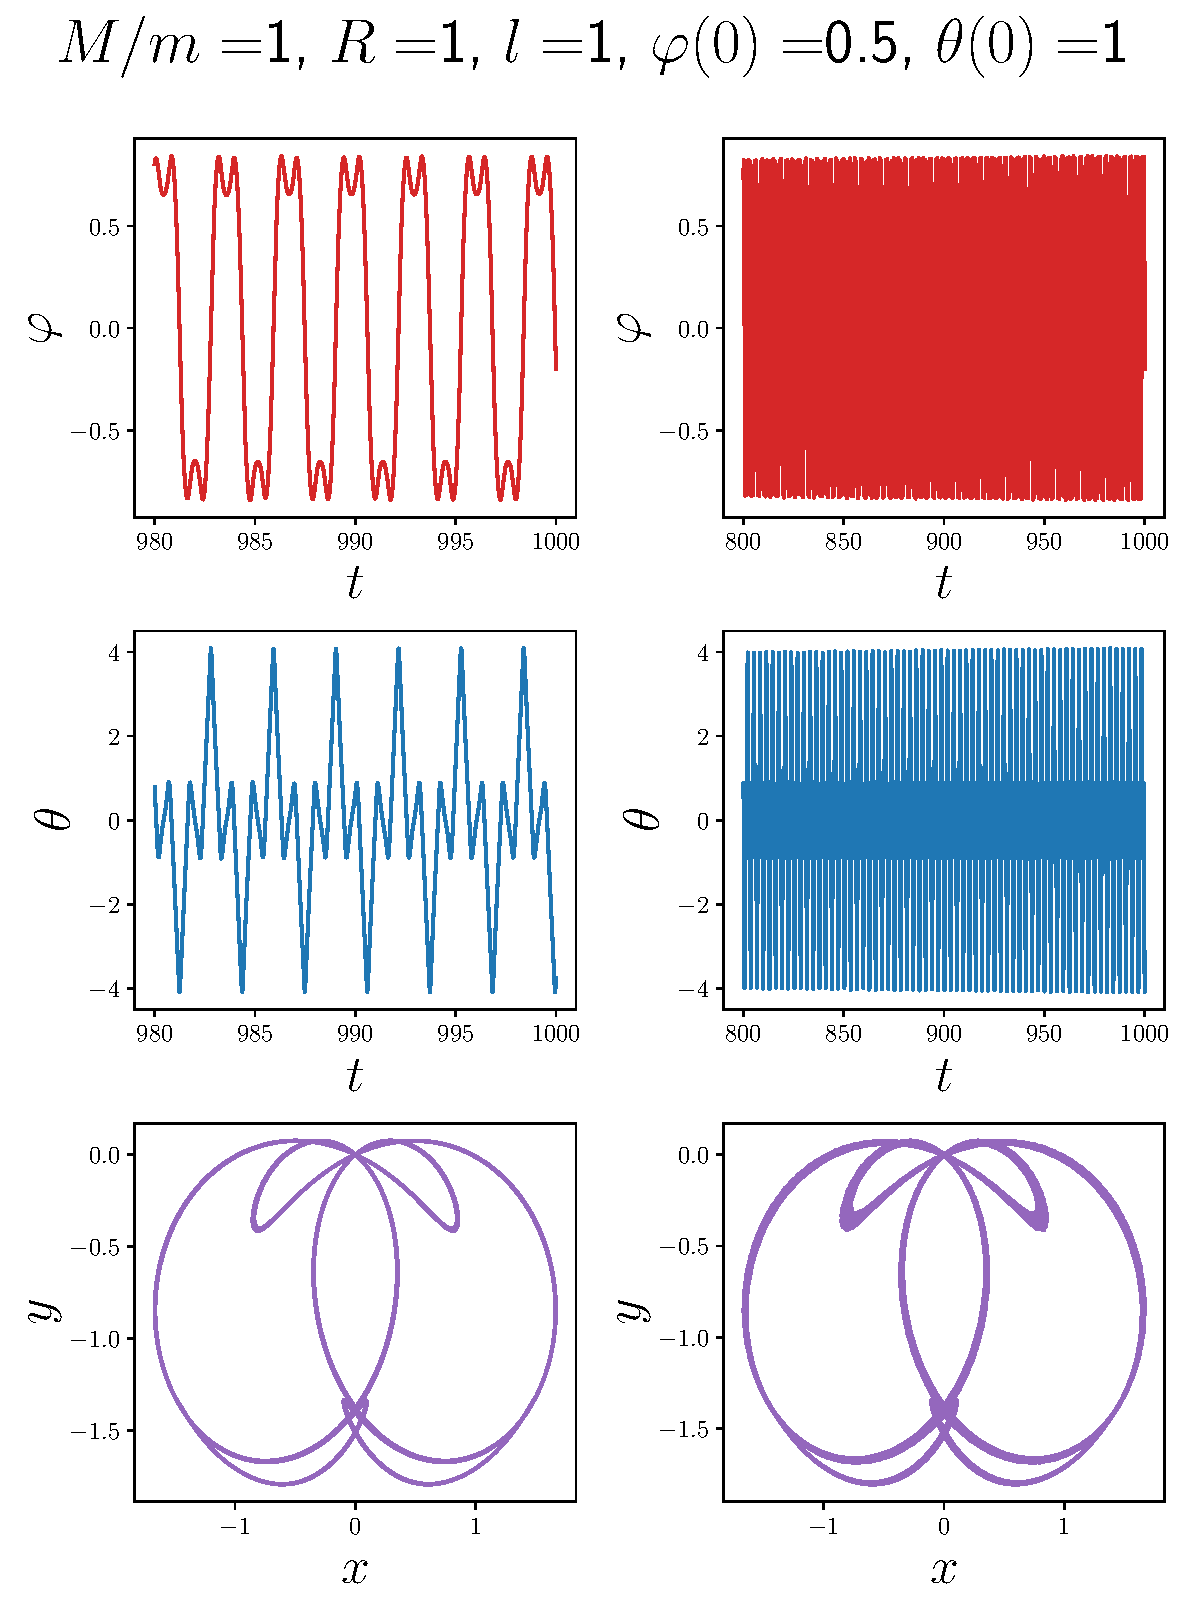
\includegraphics{../figures/2}}
	\makebox[\textwidth][c]{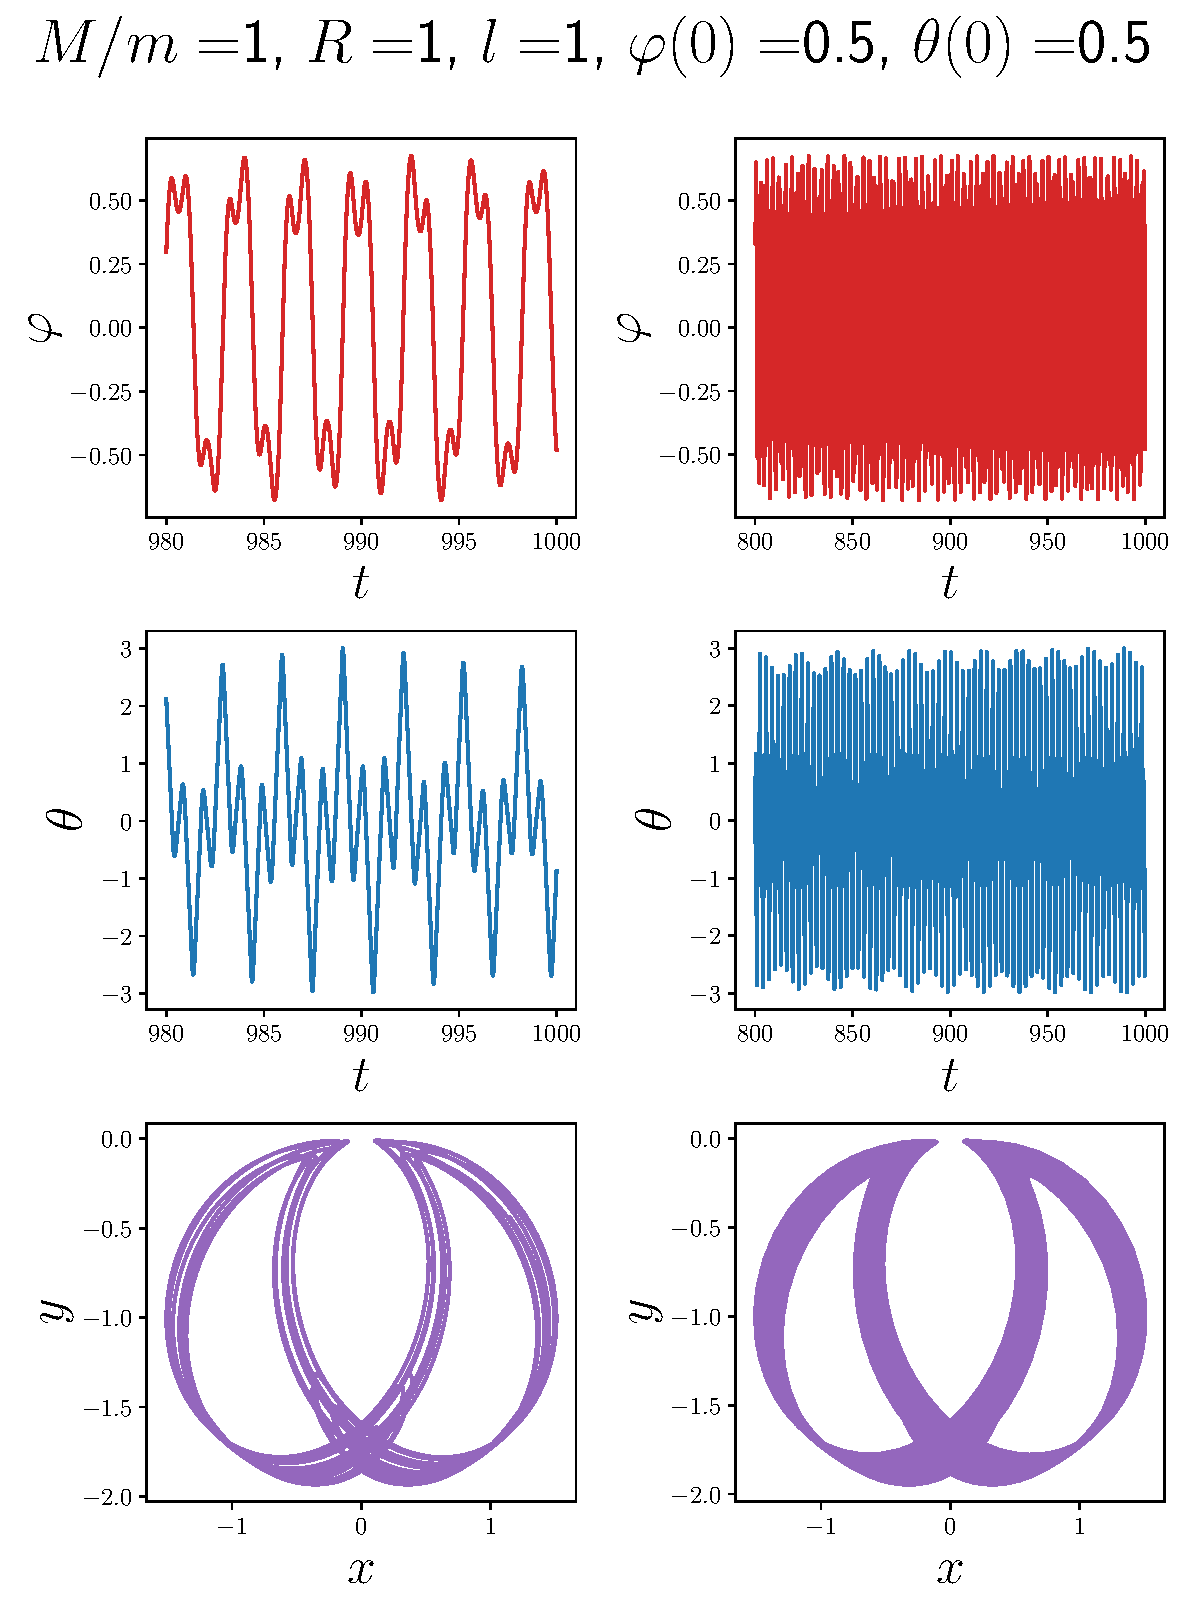
\includegraphics{../figures/3}}
	\makebox[\textwidth][c]{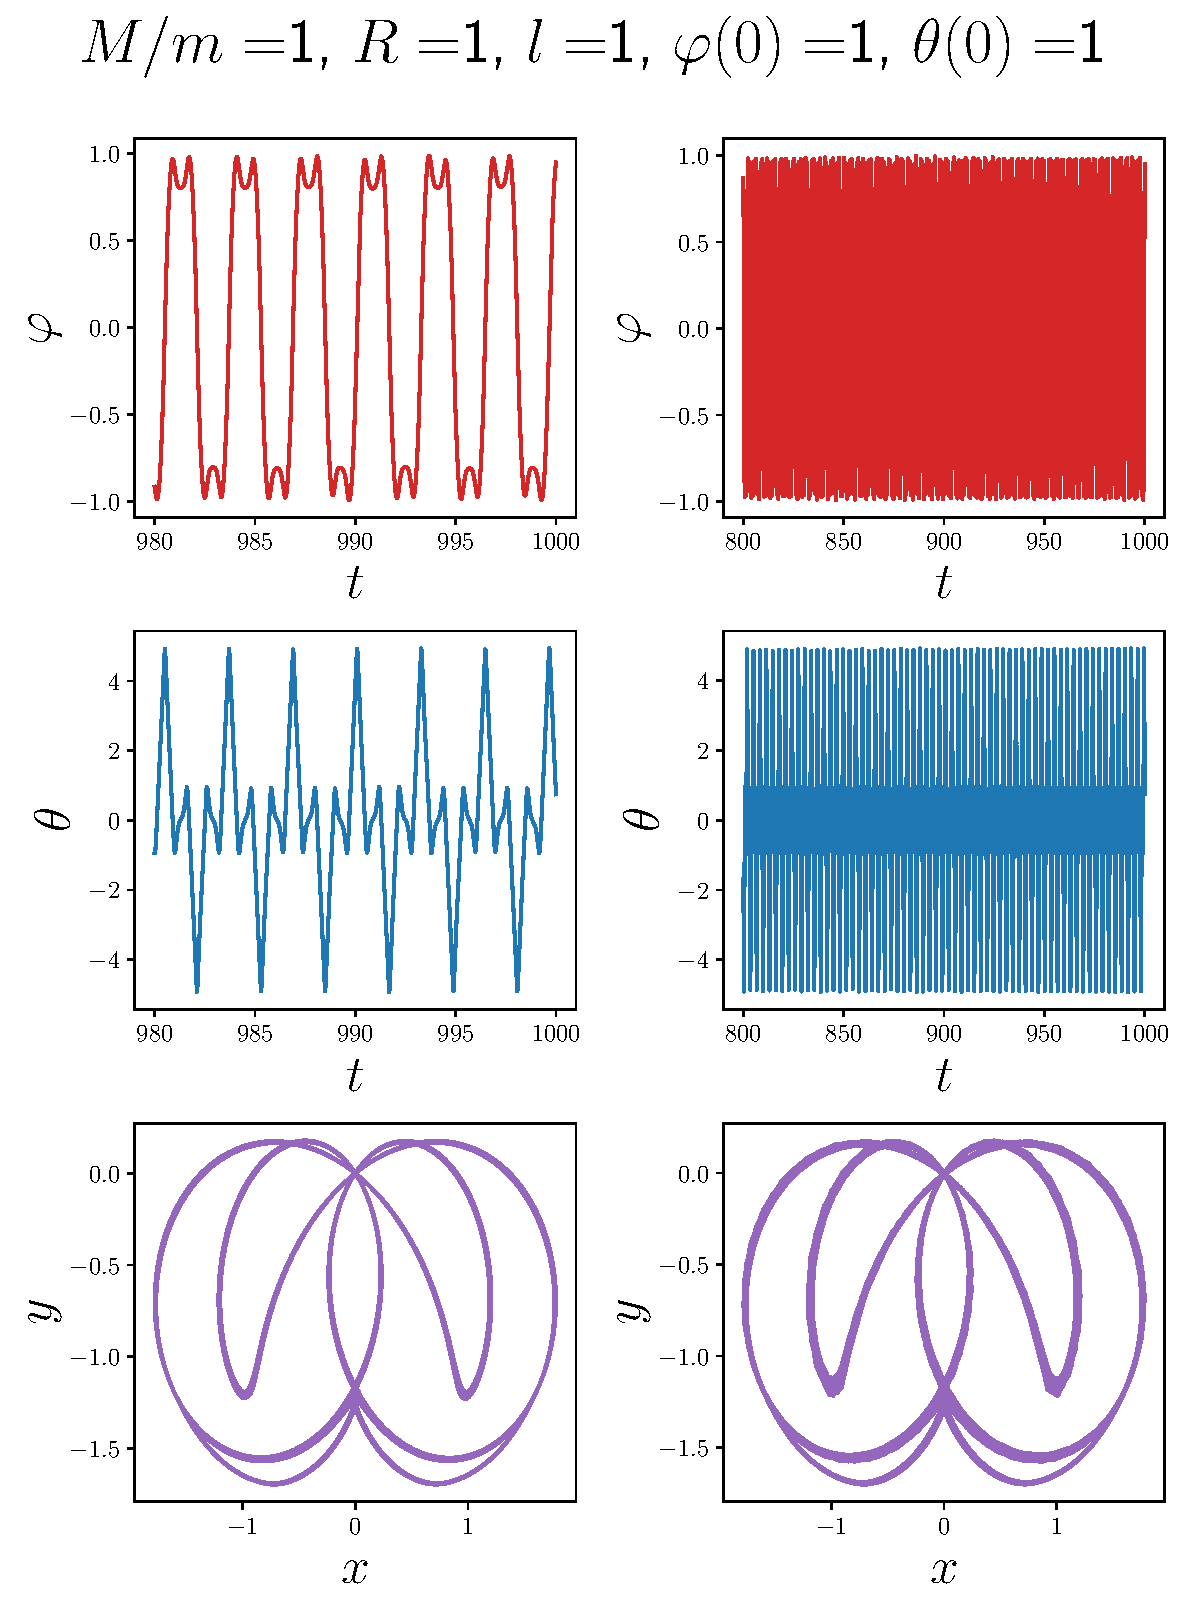
\includegraphics{../figures/4}}
	\makebox[\textwidth][c]{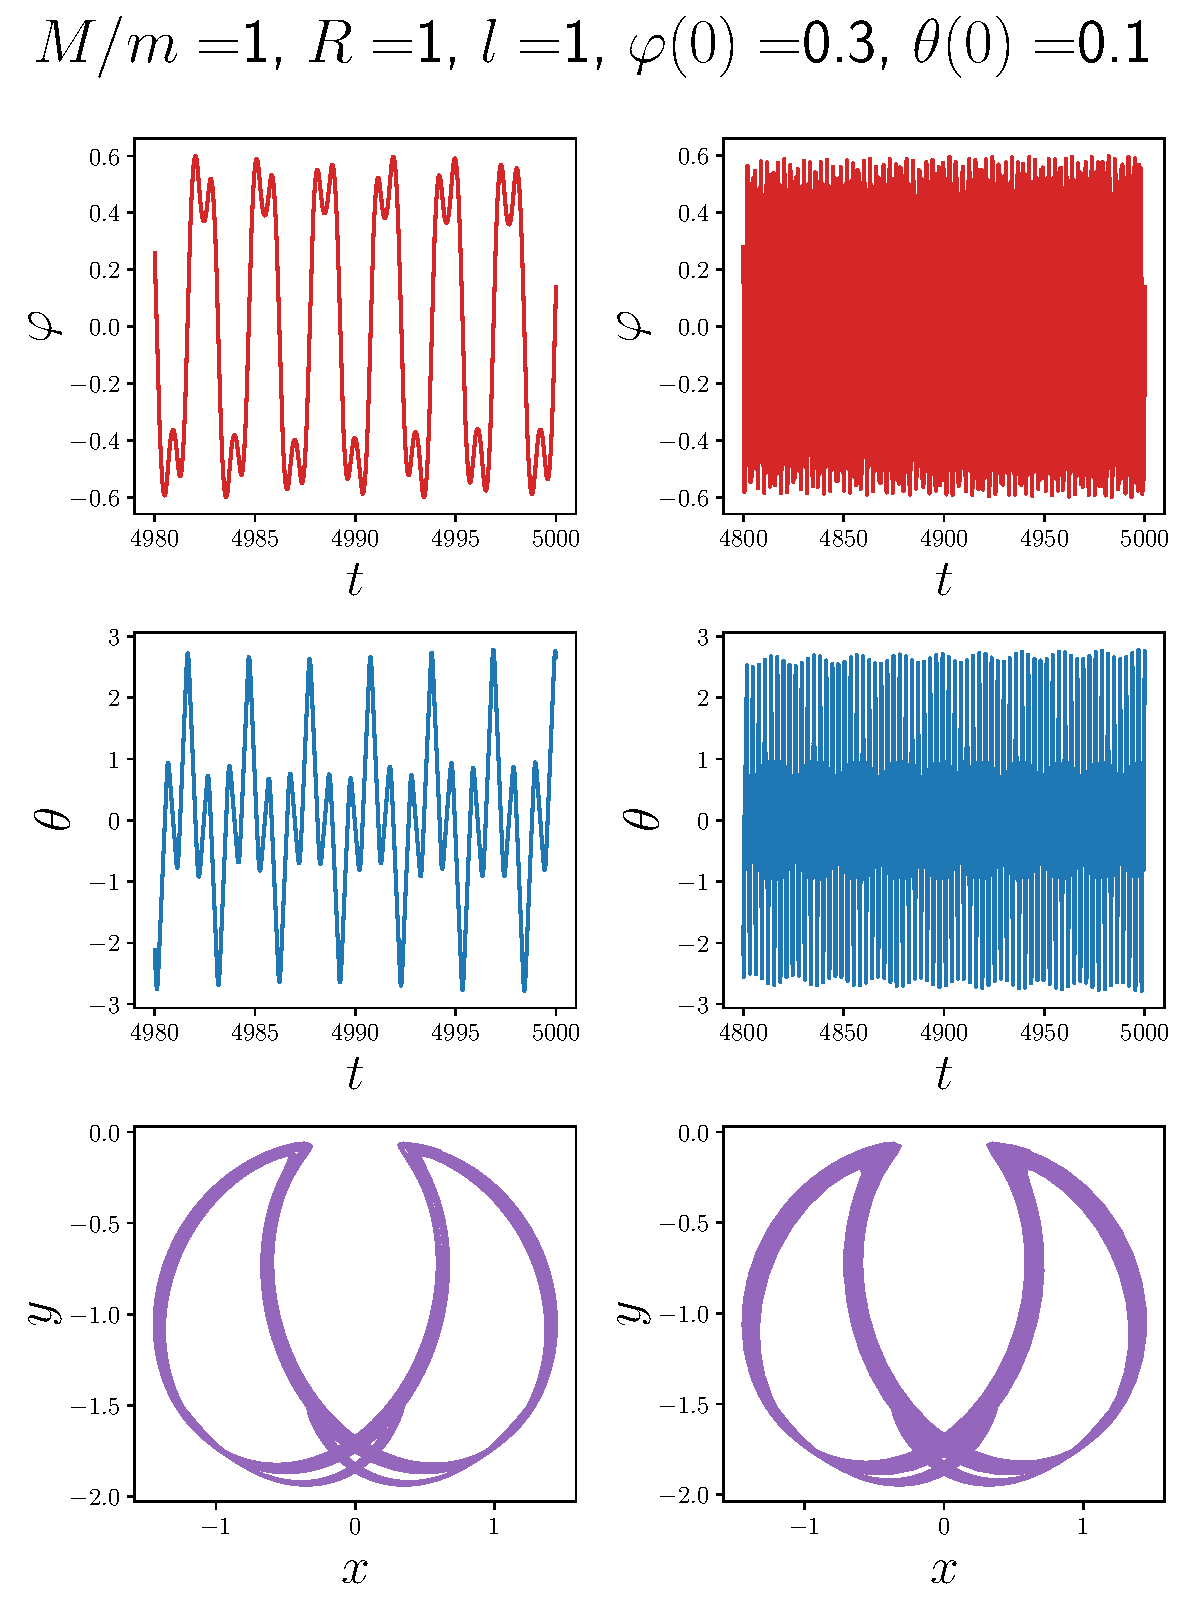
\includegraphics{../figures/5}}
	\makebox[\textwidth][c]{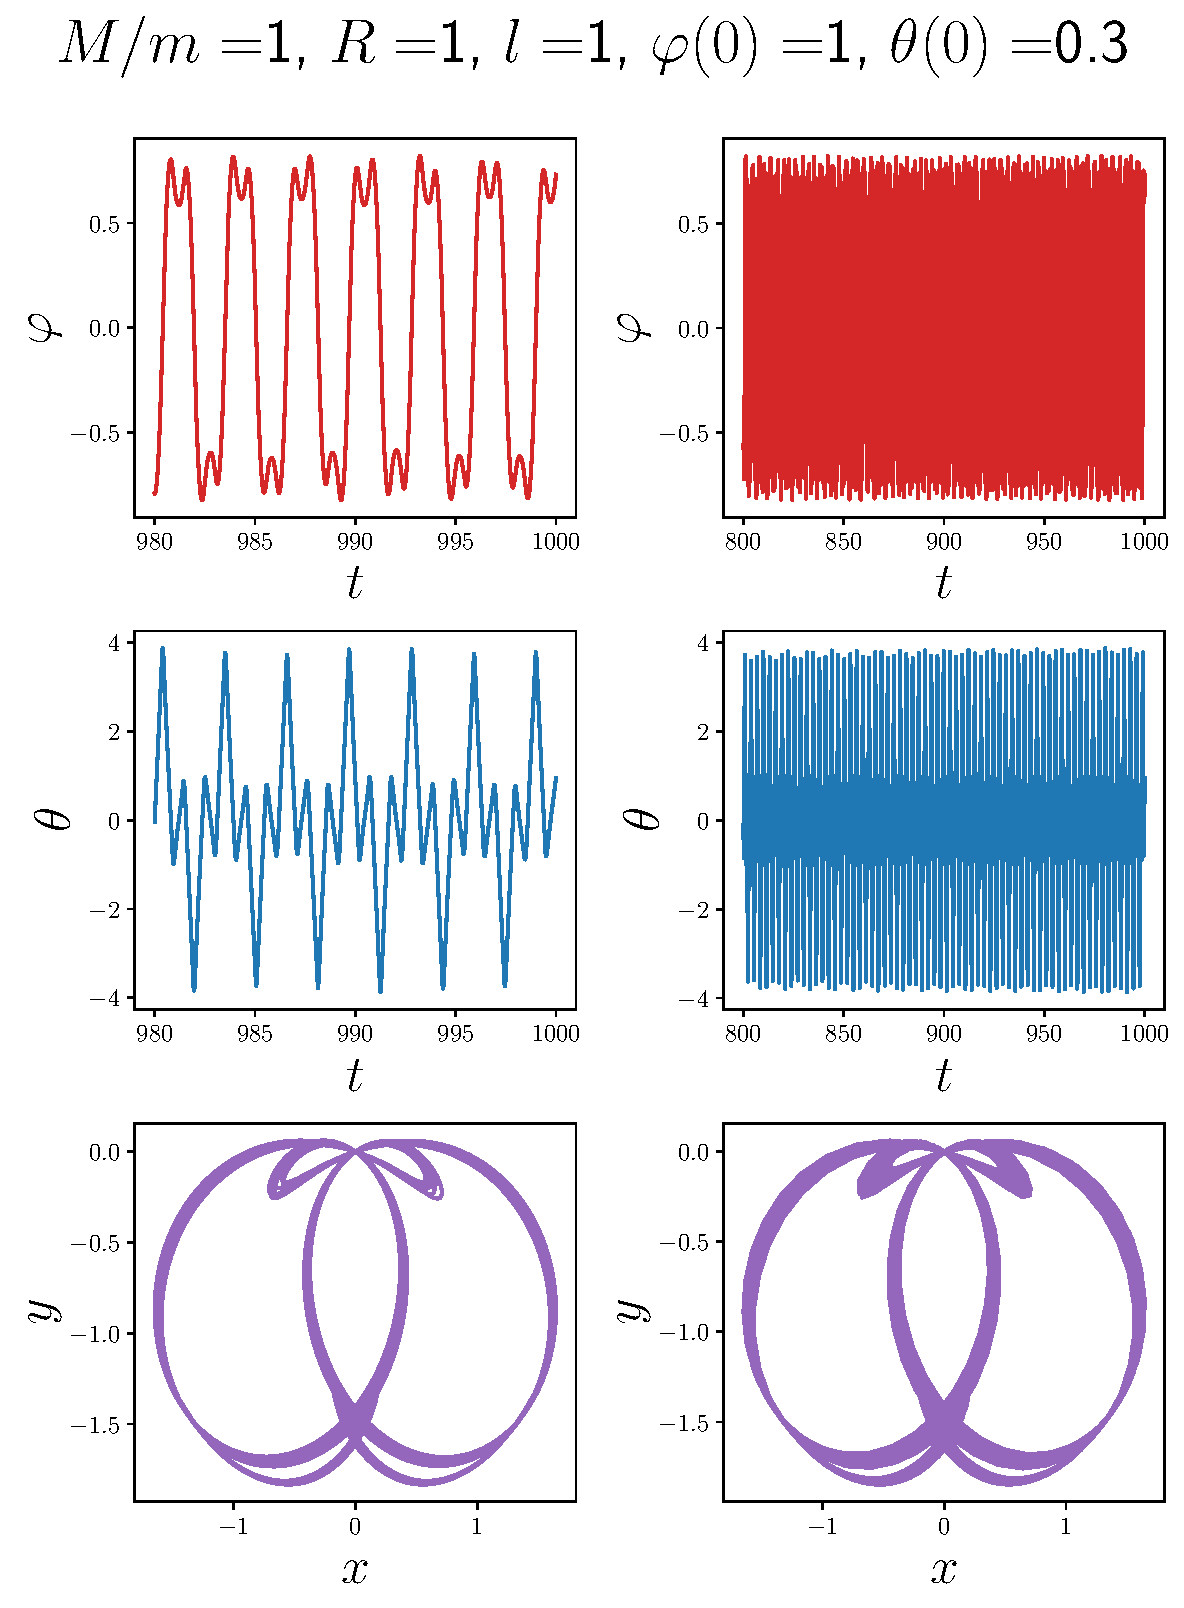
\includegraphics{../figures/6}}
	\makebox[\textwidth][c]{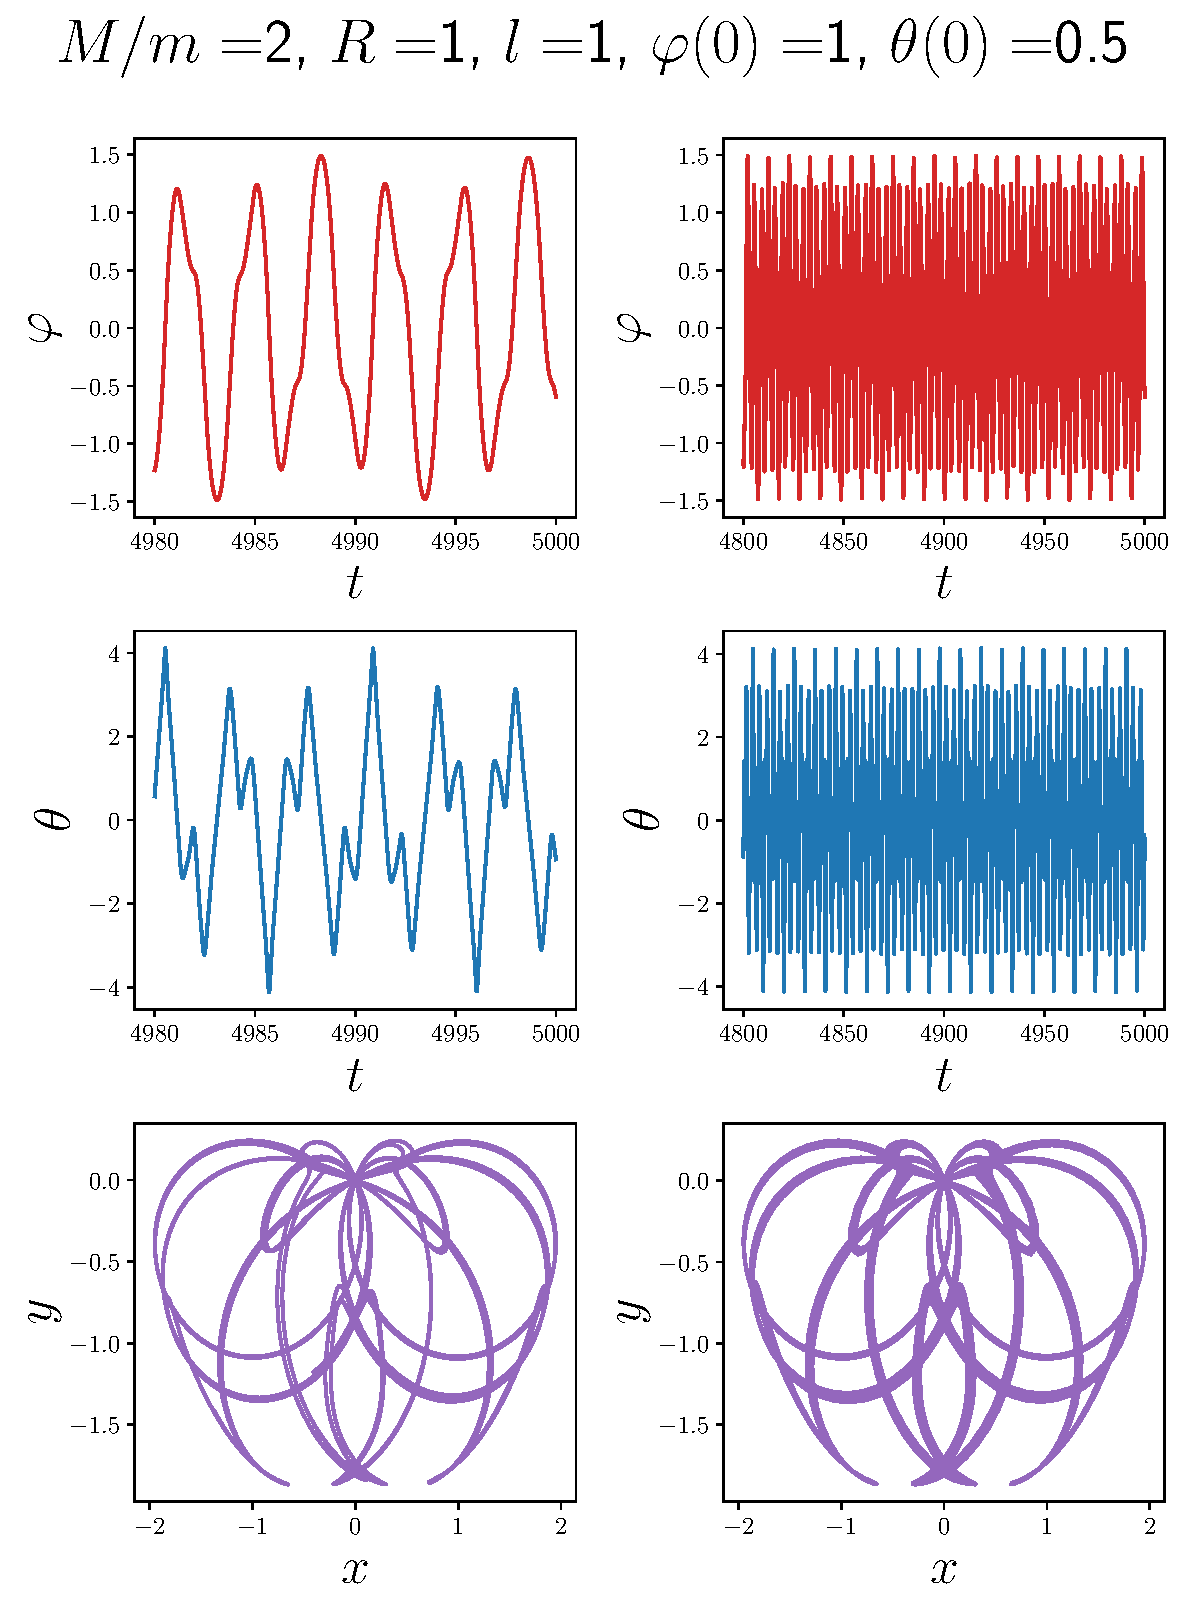
\includegraphics{../figures/7}}
	\makebox[\textwidth][c]{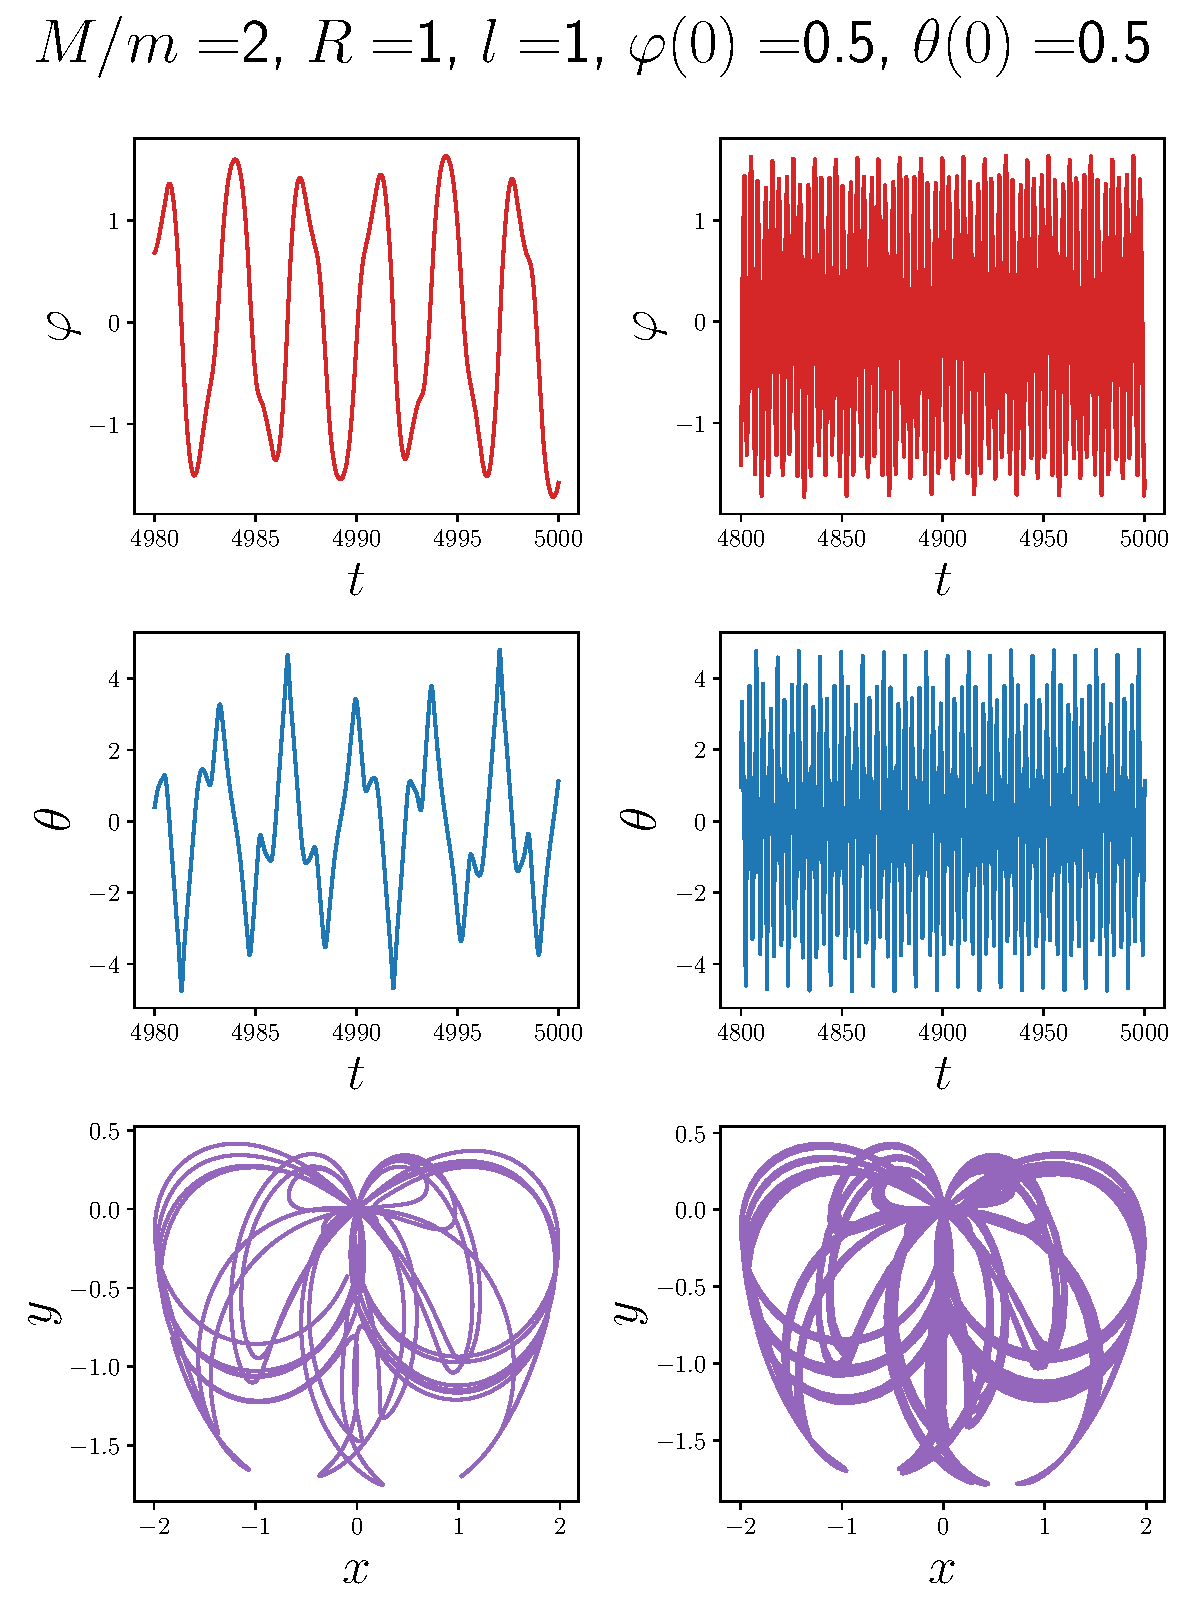
\includegraphics{../figures/8}}
	\makebox[\textwidth][c]{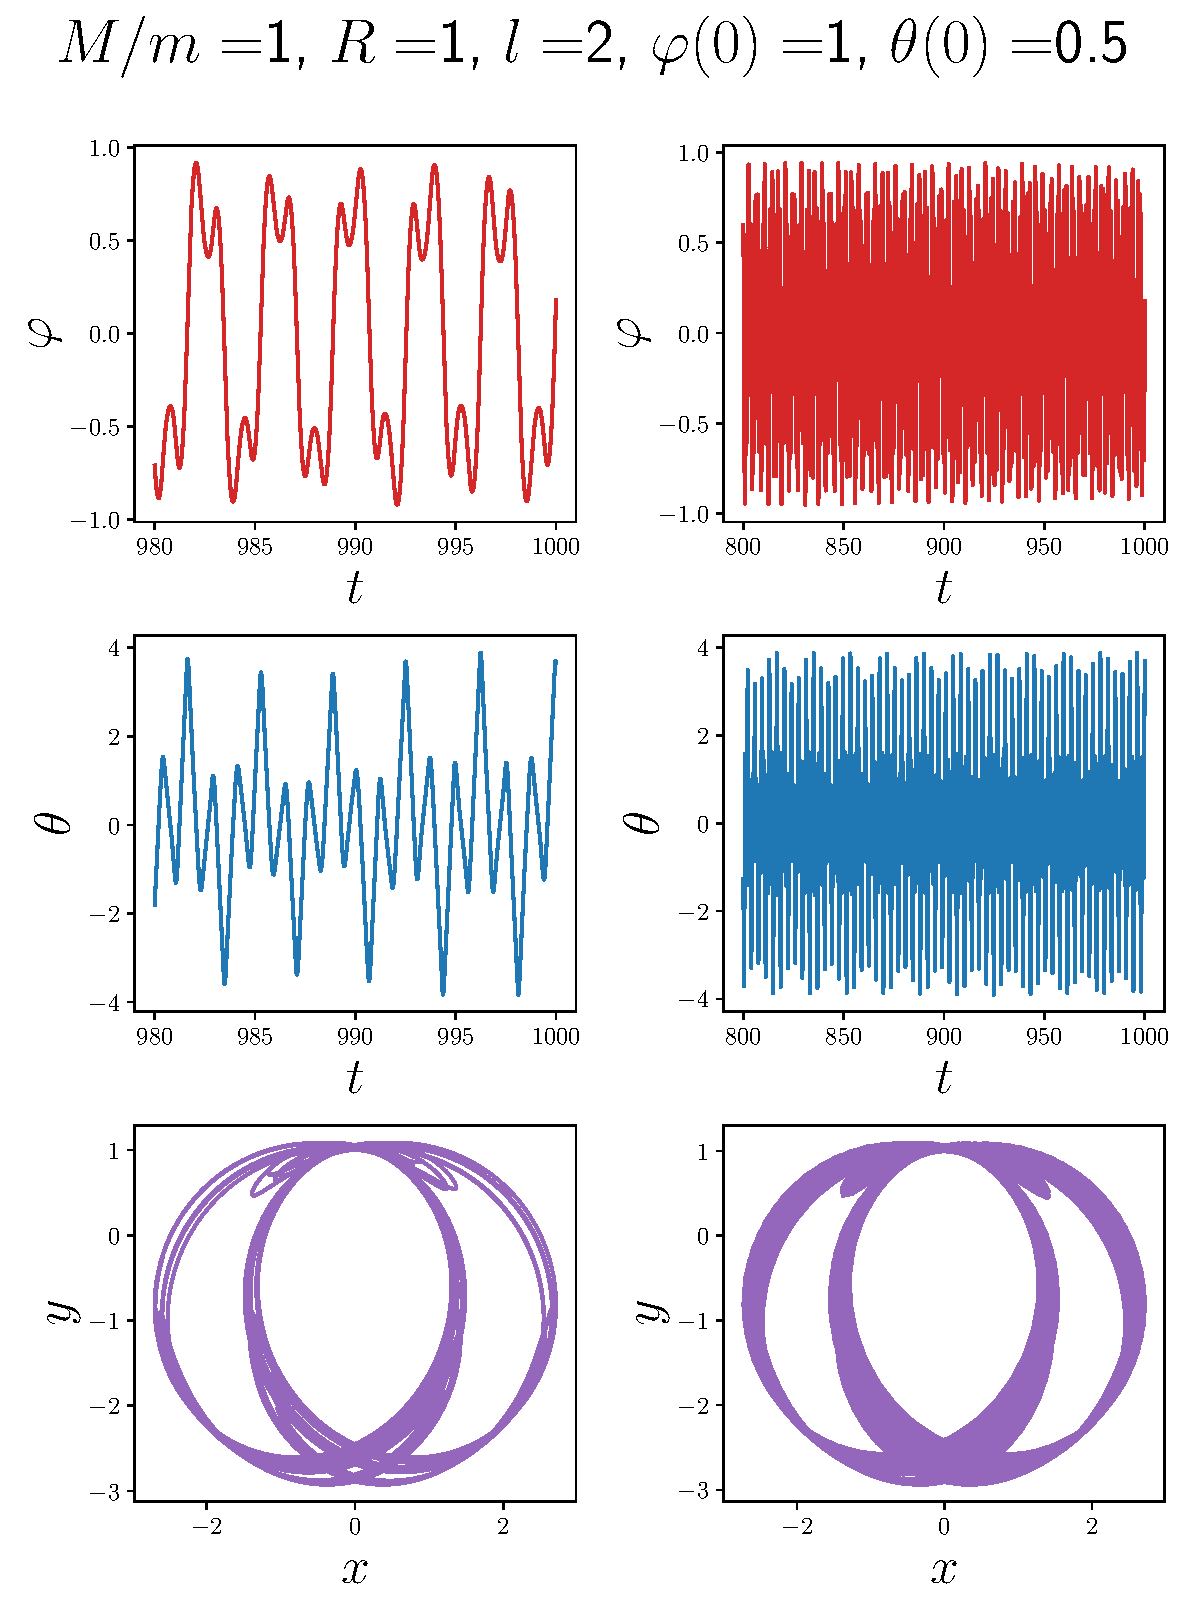
\includegraphics{../figures/9}}
	\makebox[\textwidth][c]{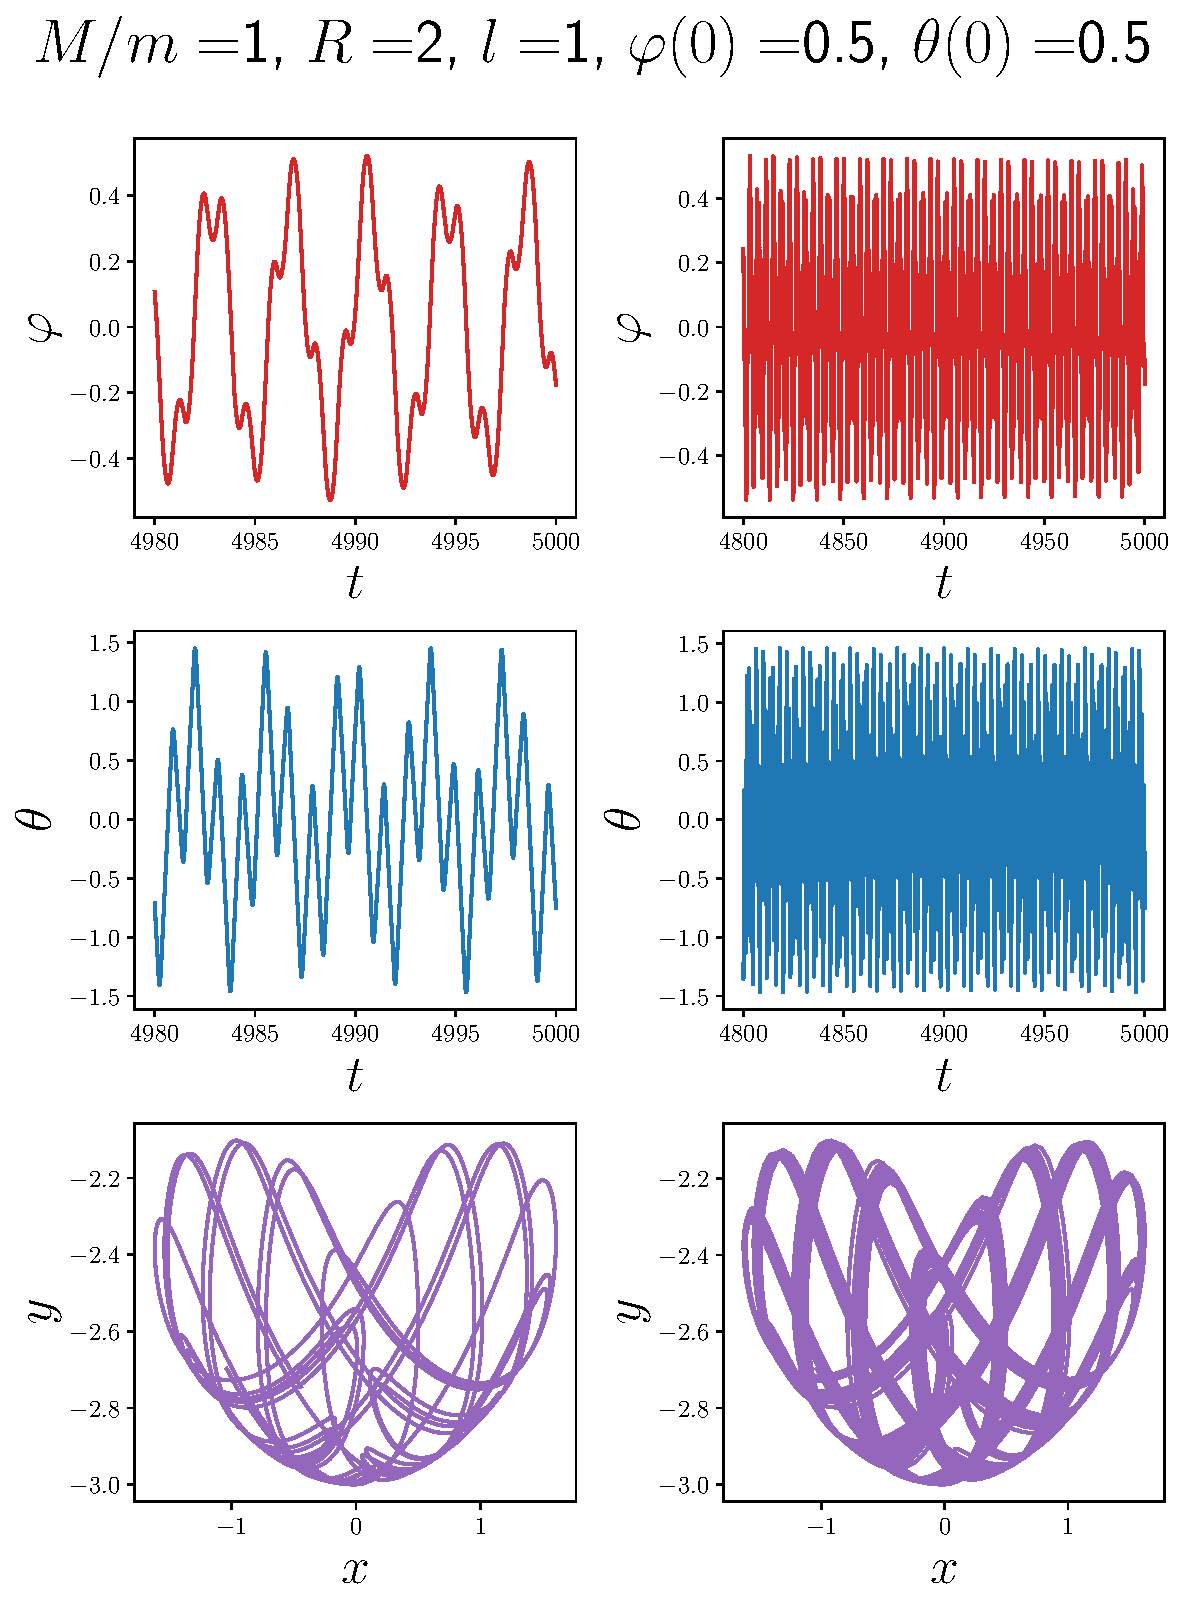
\includegraphics{../figures/10}}
	\makebox[\textwidth][c]{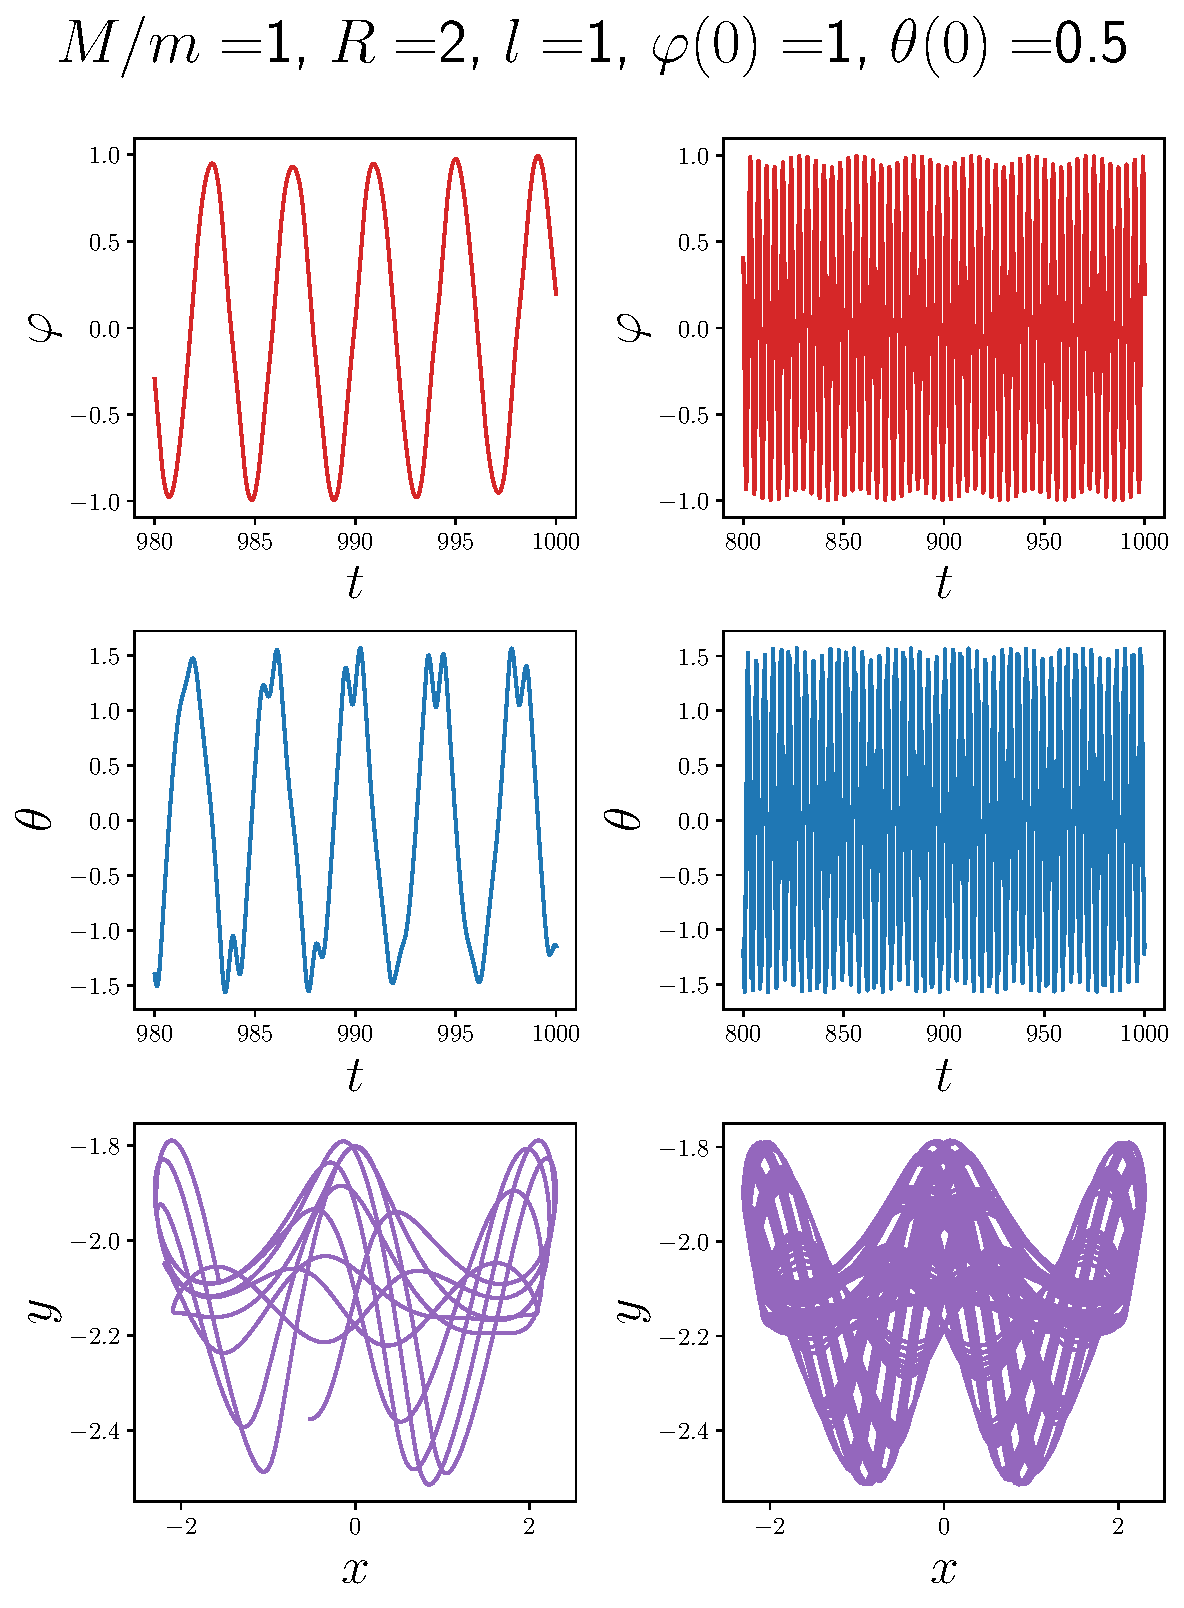
\includegraphics{../figures/11}}
	\makebox[\textwidth][c]{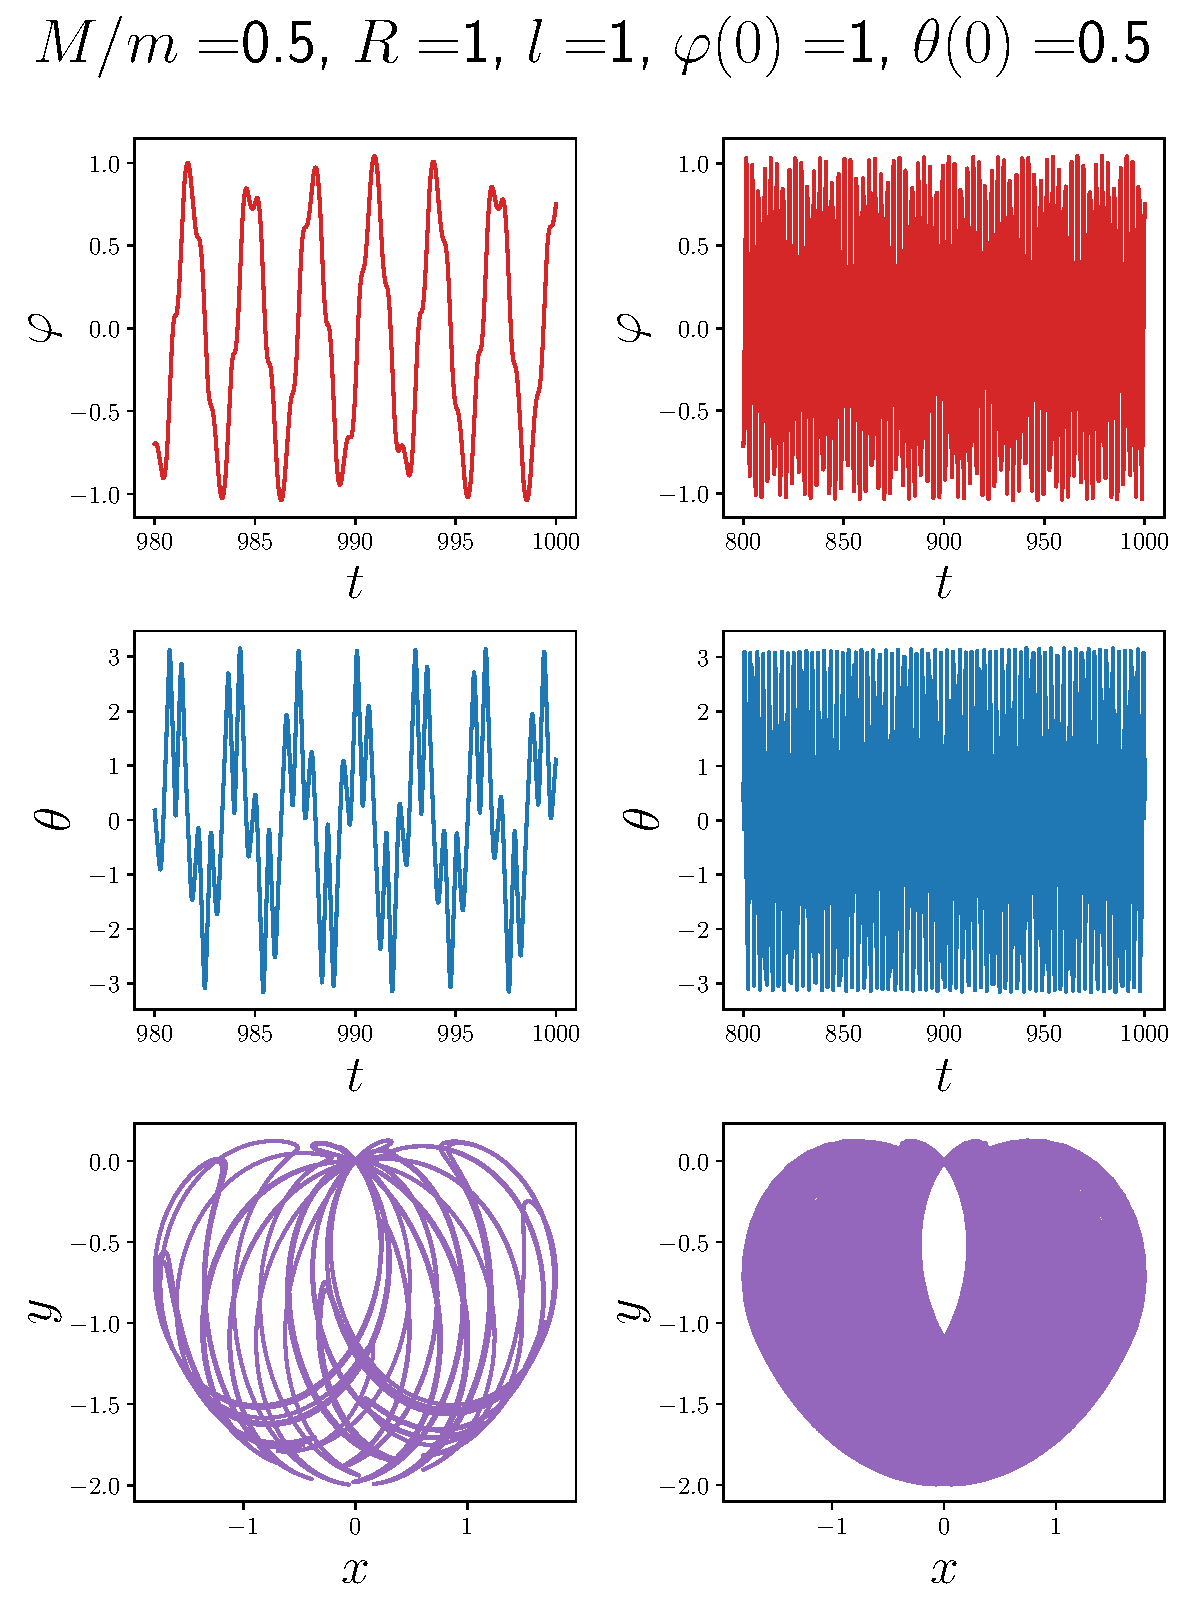
\includegraphics{../figures/12}}
	\makebox[\textwidth][c]{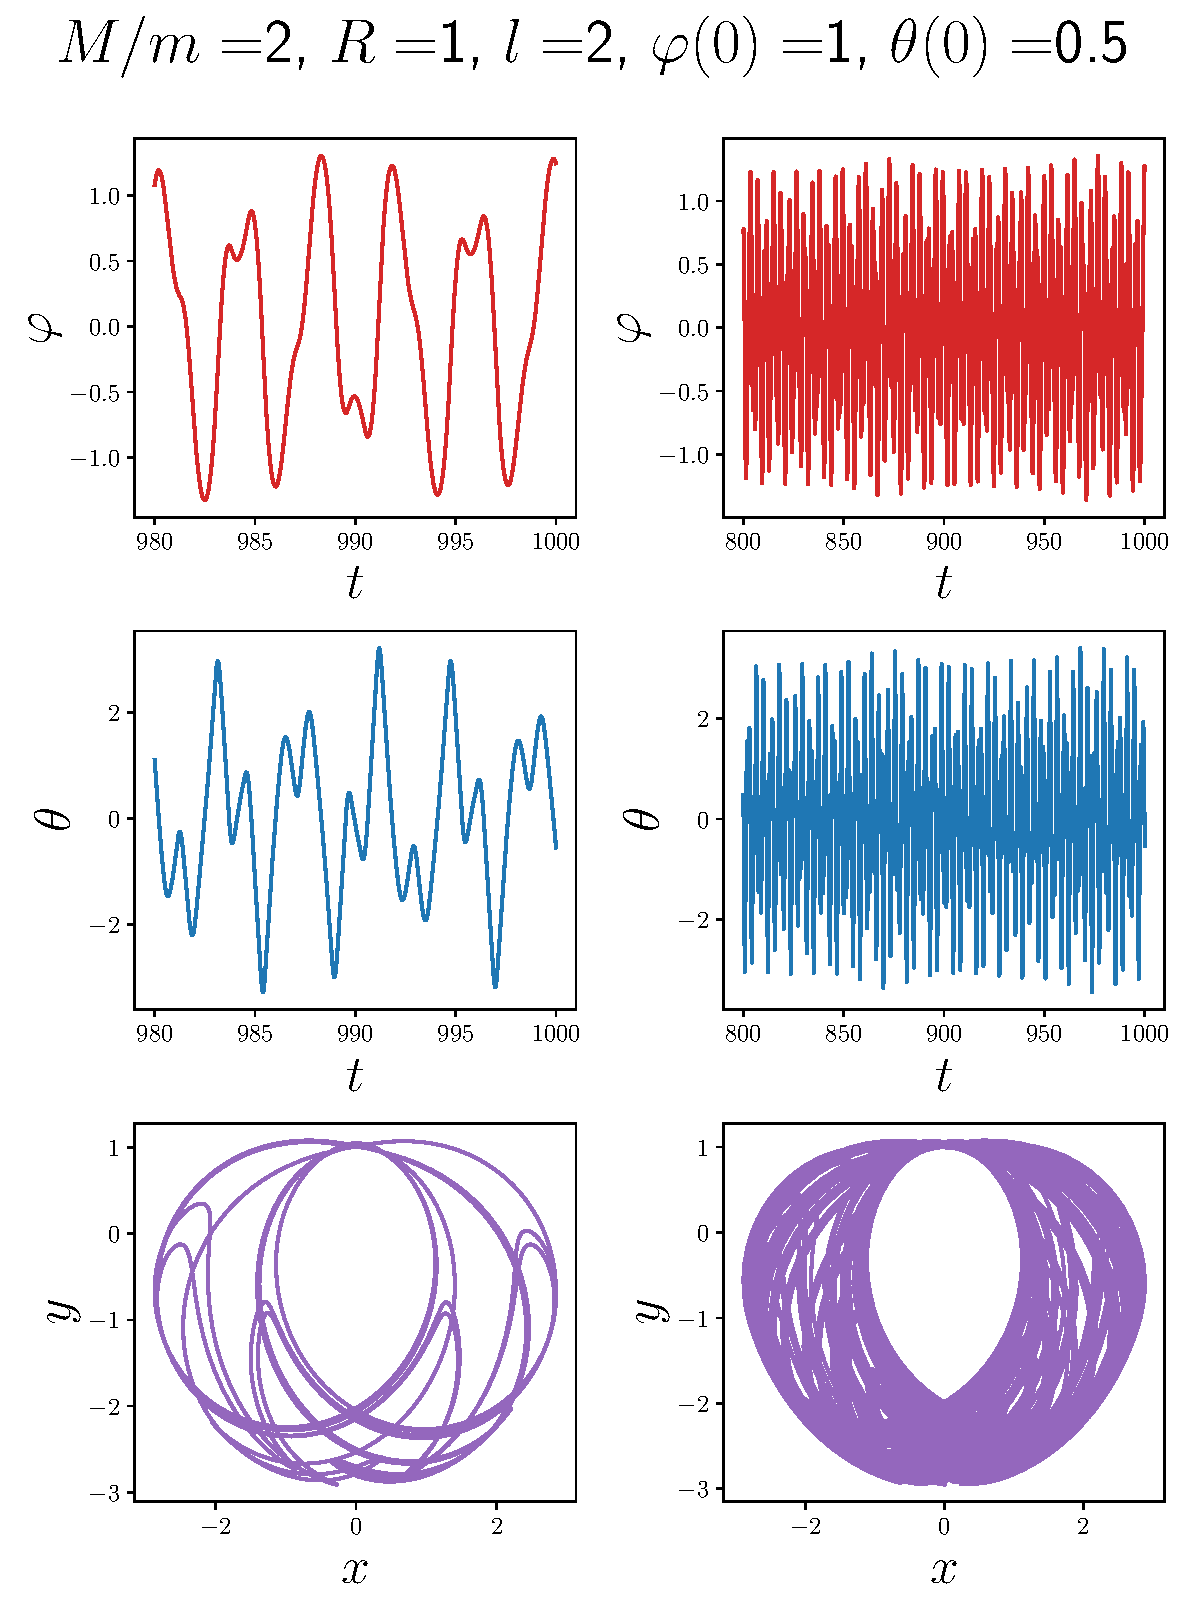
\includegraphics{../figures/13}}
	\makebox[\textwidth][c]{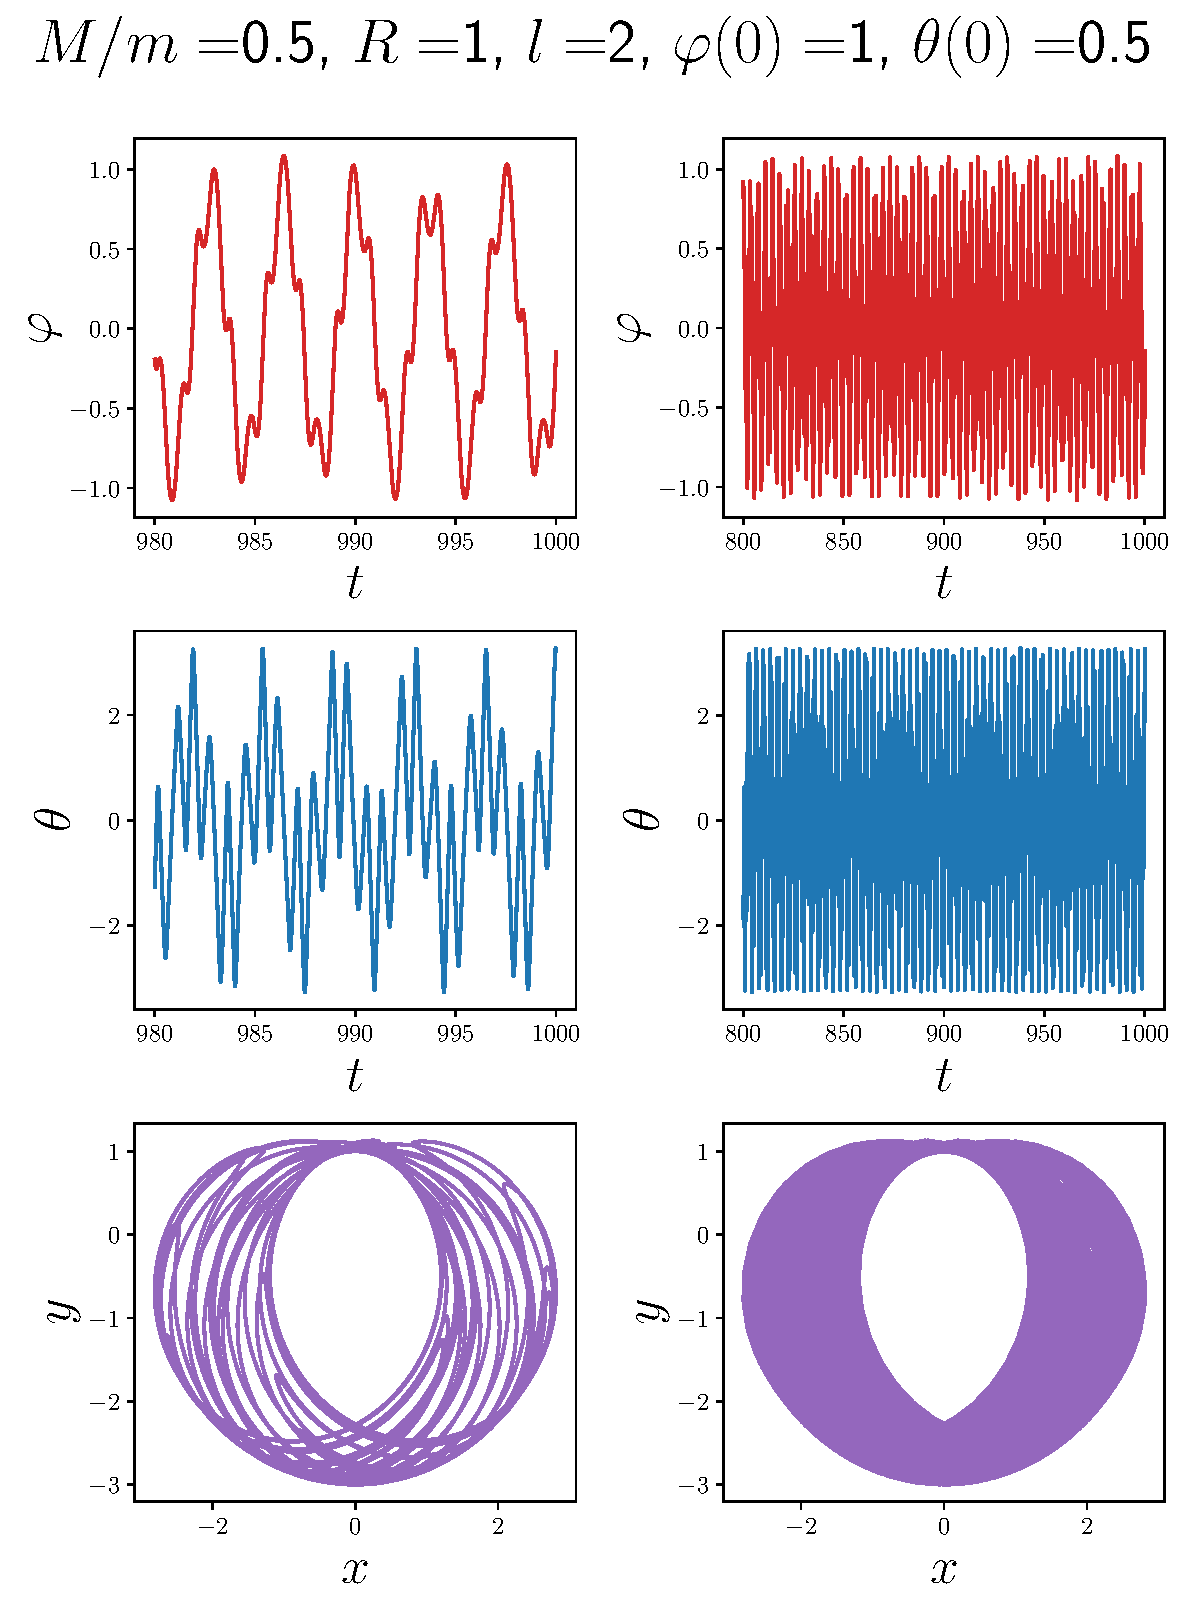
\includegraphics{../figures/14}}
	\makebox[\textwidth][c]{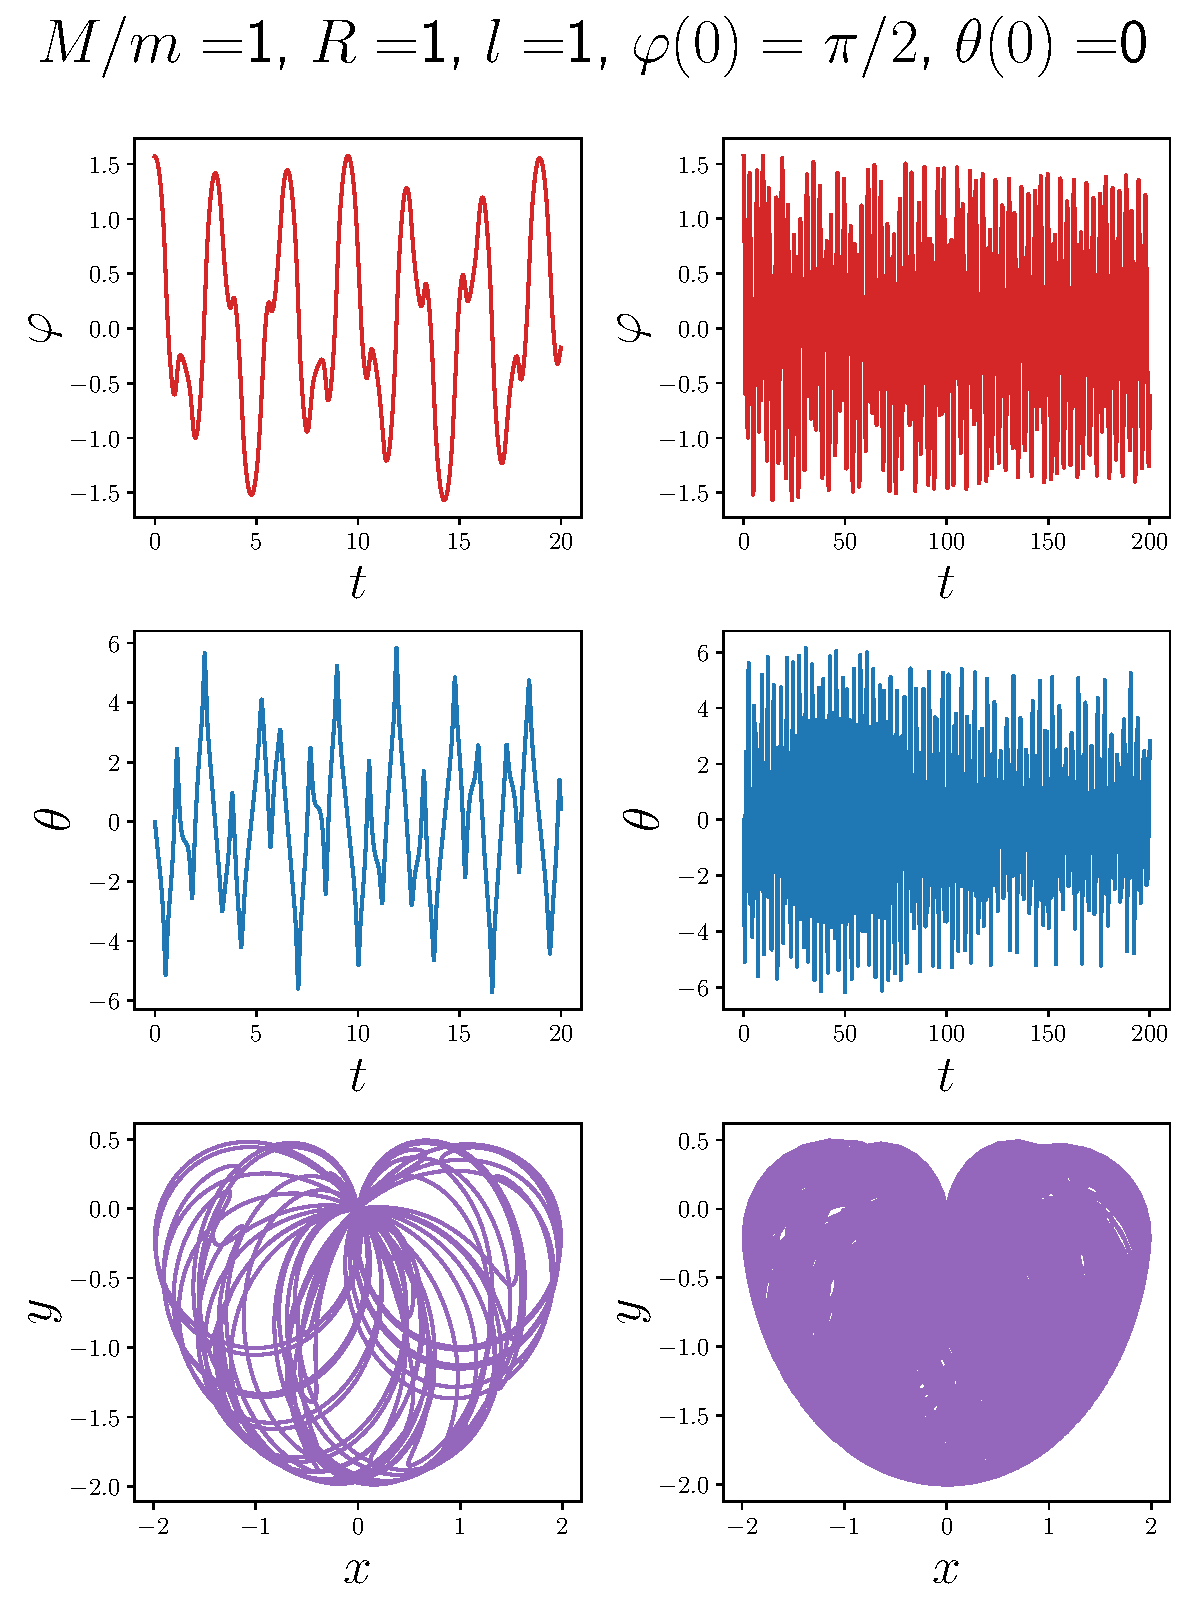
\includegraphics{../figures/15}}
	\makebox[\textwidth][c]{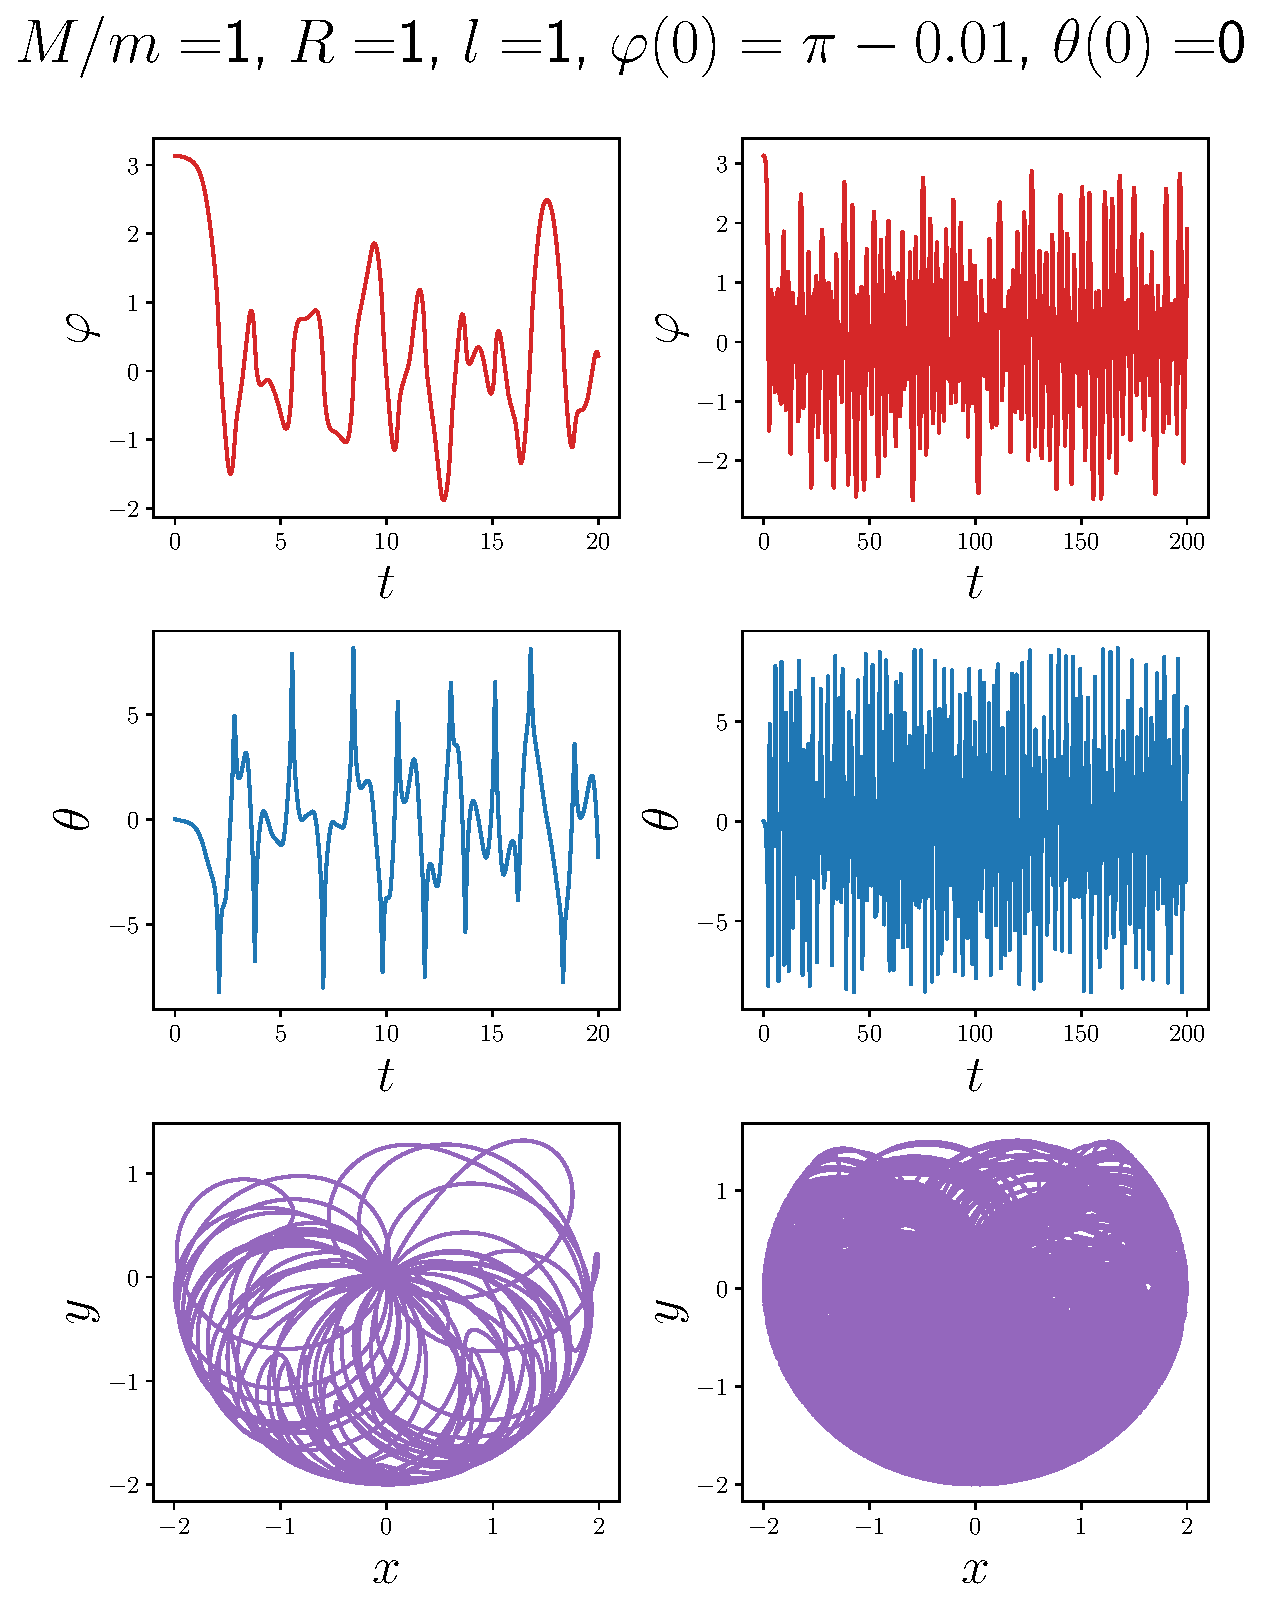
\includegraphics{../figures/16}}
	\restoregeometry
\end{document}